%!TEX program = xelatex
\documentclass[11pt,a4paper]{ctexart}

\usepackage{amsmath,amssymb,amsfonts}
\usepackage{bm}
\usepackage{graphicx}
\usepackage{booktabs}
\usepackage{multirow}
\usepackage{float}
\usepackage{geometry}
\usepackage{fancyhdr}
\usepackage{caption}
\usepackage{subcaption}
\usepackage{array}
\usepackage{enumitem}
\usepackage[ruled,linesnumbered]{algorithm2e}
\usepackage{hyperref}
\usepackage{listings}
\usepackage{xcolor}

\geometry{left=2.4cm,right=2.4cm,top=2.5cm,bottom=2.5cm}
\graphicspath{{figs/}}

\makeatletter
% 紧凑目录：去掉节前大间距，二级目录缩进显示
\renewcommand*\l@section{\@dottedtocline{1}{0em}{2.2em}}
\renewcommand*\l@subsection{\@dottedtocline{2}{2.2em}{3.2em}}
\makeatother

\hypersetup{colorlinks=true,linkcolor=black,citecolor=blue,urlcolor=blue}
\captionsetup[figure]{font=small,labelfont=bf}
\captionsetup[table]{font=small,labelfont=bf}

\lstset{
  basicstyle=\small\ttfamily,
  breaklines=true,
  frame=single,
  numbers=left,
  numberstyle=\tiny,
  keywordstyle=\color{blue},
  commentstyle=\color{gray},
  stringstyle=\color{red},
  tabsize=4,
  showstringspaces=false
}

\pagestyle{fancy}
\fancyhf{}
\setlength{\headheight}{13.6pt}
\fancyhead[L]{\small 烟幕干扰弹投放策略的建模与优化}
\fancyhead[R]{\small 2025 CUMCM A}
\fancyfoot[C]{\small\thepage}

\title{{\normalsize\bfseries 烟幕干扰弹投放策略的确定性运动学建模与全局优化研究}}
\author{}
\date{}

\begin{document}

\maketitle
\vspace{-2.8em}

\begin{abstract}
烟幕干扰弹通过形成烟幕云团截断来袭导弹对保护目标的视线，是低成本、高效费比的光电对抗手段。本文针对 2025 年高教社杯 A 题，在给定导弹与无人机初始态势、运动规则和云团有效半径的条件下，研究烟幕干扰弹投放策略，使得多枚烟幕干扰弹对真目标的有效遮蔽时间尽可能长。

本文首先以假目标为原点建立三维直角坐标系，根据导弹匀速直线飞行、无人机等高度匀速直线飞行、弹丸脱离后仅受重力、云团以 $3~\mathrm{m/s}$ 匀速下沉等规则，建立确定性运动学方程；随后将遮蔽问题转化为“导弹—目标”视线线段与云团中心球域的几何相交问题，给出点—线段距离的解析公式与多弹遮蔽区间并集时长计算方法，形成基础运动学与遮蔽判定模型。在此基础上，按问题复杂度分别建立单弹优化模型、同机多弹协同优化模型、多机协同优化模型和多机多弹多导弹全局优化模型：各模型以无人机航向角、飞行速度、投放时刻与引信延时为决策变量，以遮蔽时长最大化为目标，以速度范围、起爆高度和同机投放间隔不小于 $1~\mathrm{s}$ 为约束，并采用“排序 + 1 s 递增”的结构化编码保证硬约束自动满足。

\textbf{问题1}中，FY1 以 $120~\mathrm{m/s}$ 朝向假目标飞行、受领任务 $1.5~\mathrm{s}$ 后投放、$3.6~\mathrm{s}$ 后起爆，模型计算得 M1 有效遮蔽区间为 $[8.038,\ 9.448]~\mathrm{s}$，遮蔽时长为 $1.410~\mathrm{s}$，与 $0.005~\mathrm{s}$ 稠密采样交叉验证一致。\textbf{问题2}对 FY1 单弹的航向、速度、投放点与起爆点进行 4 维优化，最优策略为 $\theta=3.092~\mathrm{rad}$、$v=70.0~\mathrm{m/s}$、$t_d=0.158~\mathrm{s}$、$\tau=2.552~\mathrm{s}$，遮蔽时长提升至 $4.667~\mathrm{s}$，为问题 1 的 $3.31$ 倍。\textbf{问题3}在 FY1 同机三弹约束下进行 8 维联合优化，三弹遮蔽区间首尾衔接，并集遮蔽时长达 $7.740~\mathrm{s}$。\textbf{问题4}对 FY1、FY2、FY3 各投放一弹进行 12 维联合优化，三机遮蔽区间依次覆盖 $[5.458,\ 9.935]~\mathrm{s}$、$[12.609,\ 17.192]~\mathrm{s}$ 和 $[22.194,\ 27.469]~\mathrm{s}$，并集时长达 $14.335~\mathrm{s}$。\textbf{问题5}将 5 架无人机、每架至多 3 枚弹的投放资源分配给 M1、M2、M3 三枚导弹，建立 40 维全局优化模型，并针对种群级目标评估编写 Triton 批量 GPU 核函数、实现 GPU 批量差分进化，单代种群评估由 CPU 顺序约 $0.65~\mathrm{s}$ 降至约 $0.5~\mathrm{ms}$；最终总遮蔽时长达 $20.947~\mathrm{s}$，M1、M2、M3 分别为 $12.145~\mathrm{s}$、$4.855~\mathrm{s}$、$3.947~\mathrm{s}$，最差导弹遮蔽时长为 $3.947~\mathrm{s}$。

在模型检验方面，本文完成 13 项单元测试，覆盖几何距离、运动学、遮蔽判定、间隔编码与文件导出；对重力加速度、云团半径、最低起爆高度和圆柱目标判据进行扰动分析，结果表明云团半径增大 $1~\mathrm{m}$ 时各问题遮蔽时长约增加 $0.1\sim1.0~\mathrm{s}$，圆柱判据使问题 4、问题 5 遮蔽时长分别下降约 $3.0~\mathrm{s}$ 和 $4.9~\mathrm{s}$，模型响应符合物理直觉。综上，本文建立的确定性运动学与几何遮蔽模型能够为烟幕干扰弹投放策略提供定量决策依据，所得策略具有工程可实现性与可复现性。

\vspace{0.5em}
\noindent\textbf{关键词：}烟幕干扰弹；运动学建模；几何遮蔽判定；差分进化；GPU 并行优化
\end{abstract}
\newpage

\setcounter{tocdepth}{1}
{\small
\setlength{\baselineskip}{10.8pt}
\tableofcontents
}
\newpage

\section{引言}

\subsection{问题背景与意义}

烟幕干扰弹通过燃烧或爆炸在目标前方特定空域形成烟幕云团，从而截断来袭导弹对目标的视线，具有成本低、效费比高等优点。随着定点精确抛撒与时间引信控制技术的发展，由无人机在巡飞过程中按预设策略投放干扰弹已成为可行的对抗手段。2025 年高教社杯全国大学生数学建模竞赛 A 题要求在给定导弹与无人机初始态势的前提下，设计无人机飞行方向、飞行速度、干扰弹投放点与起爆点，使烟幕云团对真目标的有效遮蔽时间尽可能长。

该问题的本质是确定性三维运动学与几何遮挡的组合优化问题：导弹、无人机和干扰弹的运动规律完全已知，遮蔽效果只取决于“导弹—目标”视线与下沉烟幕云团之间的空间位置关系。因此，建模的关键在于精确刻画运动方程、建立可解析计算的遮蔽判定，并对连续投放参数进行高效全局优化。

\subsection{现有方法评述}

烟幕干扰效果评估通常采用光线遮蔽模型，将云团简化为具有有效半径的球体，并通过视线是否穿过云团来判定遮蔽状态；干扰弹投放策略则常借助火力规划或经验规则确定。已有研究多针对固定弹道或静止目标，较少同时考虑无人机等高度匀速飞行、弹丸重力下落、云团匀速下沉和多弹并集遮蔽等约束。在数值优化方面，差分进化（Differential Evolution, DE）\cite{storn1997} 对无梯度、非光滑目标函数具有较强全局搜索能力；Triton \cite{triton2019} 则可将高维种群的批量评估映射到 GPU 上，显著缩短大规模优化的求解时间。

\subsection{本文方法与贡献}

本文的主要工作包括：
\begin{enumerate}
  \item 建立导弹、无人机、干扰弹与烟幕云团的确定性运动学模型，给出“点—线段距离”遮蔽判定与多弹并集时长计算公式；
  \item 按问题复杂度分别建立单弹优化模型、同机多弹协同模型、多机协同模型与多机多弹多导弹全局优化模型，各模型决策变量、约束与目标函数清晰独立；
  \item 设计粗采样检测 + \texttt{brentq} 二分精化的遮蔽区间算法，兼顾优化过程中的计算速度与最终结果的 $10^{-6}~\mathrm{s}$ 量级精度；
  \item 采用结构化决策变量编码，将同一无人机两次投放至少间隔 $1~\mathrm{s}$ 的硬约束融入变量定义；
  \item 针对问题 5 的 40 维全局优化，编写 Triton 批量目标函数核函数并实现 GPU 批量差分进化，单代种群评估耗时由 CPU 顺序评估的约 $0.65~\mathrm{s}$ 降至 $0.5~\mathrm{ms}$ 量级；
  \item 完成单元测试、稠密采样交叉验证、敏感性分析与三维耦合可视化，保证论文中所有数值均由代码结果直接生成。
\end{enumerate}

本文结构如下：第 2 节给出问题重述与模型假设；第 3 节定义符号；第 4 节分别建立基础运动学模型、遮蔽判定模型以及各问题的优化模型；第 5 节设计求解算法；第 6 节进行模型检验与灵敏度分析；第 7 节给出并讨论各问题结果；第 8--10 节给出结论、模型评价与参考文献；第 11 节为附录。

\section{问题重述与模型假设}

\addtocontents{toc}{\protect\setcounter{tocdepth}{2}}
\subsection{问题重述}
\addtocontents{toc}{\protect\setcounter{tocdepth}{1}}

以假目标为原点建立空间直角坐标系，水平面为 $xy$ 平面，$z$ 轴竖直向上。真目标为半径 $7~\mathrm{m}$、高 $10~\mathrm{m}$ 的圆柱，其下底面圆心为 $T=(0,200,0)$。警戒雷达发现来袭导弹时，三枚导弹 M1、M2、M3 分别位于 $(20000,0,2000)$、$(19000,600,2100)$、$(18000,-600,1900)$，速度均为 $300~\mathrm{m/s}$，沿初始位置指向假目标原点的方向匀速直线飞行。五架无人机初始位置与高度见表 \ref{tab:uav}，受领任务后可在 $70\sim140~\mathrm{m/s}$ 范围内选择等高度匀速直线飞行的速度与水平航向，且一经确定不再改变。

\begin{table}[H]
\centering
\caption{无人机初始位置与飞行高度}
\label{tab:uav}
\begin{tabular}{lccc}
\toprule
无人机 & $x~\mathrm{(m)}$ & $y~\mathrm{(m)}$ & $z~\mathrm{(m)}$ \\
\midrule
FY1 & 17800 & 0 & 1800 \\
FY2 & 12000 & 1400 & 1400 \\
FY3 & 6000 & $-3000$ & 700 \\
FY4 & 11000 & 2000 & 1800 \\
FY5 & 13000 & $-2000$ & 1300 \\
\bottomrule
\end{tabular}
\end{table}

烟幕干扰弹脱离无人机后仅受重力作用，起爆后瞬时形成以云团中心为球心、有效半径 $10~\mathrm{m}$ 的球状烟幕云团；云团中心以 $3~\mathrm{m/s}$ 匀速下沉，起爆后 $20~\mathrm{s}$ 内有效。同一无人机投放两枚弹至少间隔 $1~\mathrm{s}$。需依次求解五个问题：固定策略遮蔽时长（问题 1）、单弹优化（问题 2）、FY1 三弹优化（问题 3）、三机各一弹优化（问题 4）、五机至多十五弹对三导弹的总体优化（问题 5）。

\addtocontents{toc}{\protect\setcounter{tocdepth}{2}}
\subsection{问题特征分析}
\addtocontents{toc}{\protect\setcounter{tocdepth}{1}}

在建模之前，先根据给定数据提取问题结构特征。三枚导弹的初始位置、到达时刻以及五架无人机的引信延时上限如表 \ref{tab:impact} 所示，其中引信延时上限由式 \eqref{eq:height} 反推：
\begin{equation}
  \tau_{\max}(h_k)=\sqrt{\frac{2(h_k-60)}{g}}.
  \label{eq:taumax}
\end{equation}

\begin{table}[H]
\centering
\caption{导弹到达时刻与无人机引信延时上限}
\label{tab:impact}
\small
\begin{tabular}{lccc}
\toprule
导弹 & 初始位置 (m) & 到达时刻 (s) \\
\midrule
M1 & $(20000,0,2000)$ & 67.00 \\
M2 & $(19000,600,2100)$ & 63.75 \\
M3 & $(18000,-600,1900)$ & 60.37 \\
\bottomrule
\end{tabular}
\qquad
\begin{tabular}{lcc}
\toprule
无人机 & 高度 (m) & $\tau_{\max}$ (s) \\
\midrule
FY1 & 1800 & 18.84 \\
FY2 & 1400 & 16.54 \\
FY3 & 700 & 11.43 \\
FY4 & 1800 & 18.84 \\
FY5 & 1300 & 15.91 \\
\bottomrule
\end{tabular}
\end{table}

由表 \ref{tab:impact} 可得到三点结构特征：M1 窗口最长且 FY1、FY4 高度最高，拥有最大的可布设时间轴；M3 最早到达且 FY3 高度最低，是资源竞争中的薄弱环节；同一无人机航向与速度被多弹共享，只能通过投放时刻与引信延时错开，这决定了模型四、模型六必须采用结构化时序编码。这些特征将在结果分析中用于解释最优策略形态。

\addtocontents{toc}{\protect\setcounter{tocdepth}{2}}
\subsection{模型假设}
\addtocontents{toc}{\protect\setcounter{tocdepth}{1}}

为将实际问题转化为可计算的数学模型，本文作如下假设，并说明其合理性：

\begin{enumerate}[label=\textbf{假设\arabic*.}]
  \item $t=0$ 为警戒雷达发现目标、控制中心指派任务的时刻，无人机可瞬时完成航向调整。\textit{合理性：}指挥决策时间相对飞行过程很短，题目未给出调整耗时。
  \item 导弹沿初始位置指向假目标原点的直线匀速飞行，不考虑减速、转弯与高度变化。\textit{合理性：}题目明确导弹速度恒定、方向直指假目标。
  \item 无人机受领任务后以选定航向与速度等高度匀速直线飞行，航向速度一经确定不再改变；同一无人机投放的弹共享航向与速度。\textit{合理性：}题目明确约束。
  \item 干扰弹脱离无人机后仅受重力，起爆前无姿态与推力控制；起爆点由投放时刻与引信延时唯一确定。\textit{合理性：}题目未提供空气阻力等数据，符合“不引入题目未给物理”的原则。
  \item 遮蔽判定（基准模型）：导弹在时刻 $t$ 到真目标中心 $T$ 的视线线段被云团遮挡，当且仅当该线段到云团中心的最近距离不大于 $10~\mathrm{m}$。\textit{合理性：}云团中心 $10~\mathrm{m}$ 范围内有效是题目给出的试验结论。
  \item 圆柱目标扩展模型：以“导弹到圆柱表面任意点的视线均被遮挡”为更严格判据，用于稳健性检验。\textit{合理性：}真目标为圆柱，考虑全部表面点更保守。
  \item 为保证云团 $20~\mathrm{s}$ 下沉期间不接地，起爆高度应不小于 $60~\mathrm{m}$；否则该弹视为无效。\textit{合理性：}由下沉速度 $3~\mathrm{m/s} \times 20~\mathrm{s}=60~\mathrm{m}$ 得出。
  \item 多枚弹的遮蔽时间可不相连，总有效遮蔽时长按时间并集计算。\textit{合理性：}题目明确说明。
\end{enumerate}

\section{符号说明与变量定义}

本文主要符号及其含义如表 \ref{tab:symbol} 所示。除特别说明外，向量用粗体表示，标量用斜体表示，单位为国际单位制。

\begin{table}[H]
\centering
\caption{主要符号说明}
\label{tab:symbol}
\small
\begin{tabular}{lll}
\toprule
符号 & 含义 & 单位 \\
\midrule
$\bm{P}_{m0},\ \bm{u}_m$ & 导弹 $m$ 的初始位置、单位方向向量 & m, --- \\
$v_m=300$ & 导弹飞行速度 & m/s \\
$\bm{U}_{k0},\ h_k$ & 无人机 $k$ 的初始位置、飞行高度 & m \\
$\theta_k,\ v_k$ & 无人机 $k$ 的水平航向角、飞行速度 & rad, m/s \\
$t_{dj},\ \tau_j$ & 第 $j$ 枚弹的投放时刻、引信延时 & s \\
$\bm{D}_j,\ \bm{E}_j$ & 第 $j$ 枚弹的投放点、起爆点 & m \\
$\bm{C}_j(t)$ & 第 $j$ 个云团在时刻 $t$ 的中心位置 & m \\
$\bm{T}=(0,200,0)$ & 真目标下底面圆心 & m \\
$R=10$ & 云团有效遮蔽半径 & m \\
$g=9.8$ & 重力加速度 & m/s$^2$ \\
$T_{\mathrm{impact},m}$ & 导弹 $m$ 到达假目标的时刻 & s \\
$d_{jm}(t)$ & 时刻 $t$ 云团 $j$ 中心到视线线段的距离 & m \\
$S_{jm}$ & 云团 $j$ 对导弹 $m$ 的遮蔽时间集合 & s \\
$T_m$ & 导弹 $m$ 的有效遮蔽时长 & s \\
\bottomrule
\end{tabular}
\end{table}

\section{模型建立}

本节按照“先基础、后扩展、再逐问题细化”的思路，将问题拆分为七个相互衔接的模型：模型一建立通用运动学基础模型；模型二建立遮蔽判定与并集时长模型；模型三至模型六分别为问题 2--5 的优化模型；模型七为圆柱目标扩展模型。

\addtocontents{toc}{\protect\setcounter{tocdepth}{2}}
\subsection{模型一：通用运动学基础模型}
\addtocontents{toc}{\protect\setcounter{tocdepth}{1}}

该模型回答“导弹、无人机、干扰弹和云团在任意时刻位于何处”，是全部后续模型的基础。

\subsubsection{导弹运动方程}

设导弹 $m$ 的初始位置为 $\bm{P}_{m0}=(x_{m0},y_{m0},z_{m0})$，其指向假目标原点的单位方向向量为
\begin{equation}
  \bm{u}_m = -\frac{\bm{P}_{m0}}{\|\bm{P}_{m0}\|},
  \label{eq:dir}
\end{equation}
则导弹在时刻 $t$ 的位置为
\begin{equation}
  \bm{P}_m(t) = \bm{P}_{m0} + v_m t\,\bm{u}_m, \qquad 0\le t\le T_{\mathrm{impact},m},
  \label{eq:missile}
\end{equation}
其中 $v_m=300~\mathrm{m/s}$，$T_{\mathrm{impact},m}=\|\bm{P}_{m0}\|/v_m$。式 \eqref{eq:dir} 中负号体现“指向假目标原点”的方向约束；式 \eqref{eq:missile} 为匀速直线运动，其物理含义是导弹位置随时间线性变化，仿真窗口取 $[0,T_{\mathrm{impact},m}]$。

\subsubsection{无人机与干扰弹运动方程}

设无人机 $k$ 的初始位置为 $\bm{U}_{k0}=(x_{k0},y_{k0},h_k)$，水平航向角为 $\theta_k$，速度为 $v_k$，则
\begin{equation}
  \bm{U}_k(t)=\bm{U}_{k0}+v_k t\,(\cos\theta_k,\ \sin\theta_k,\ 0).
  \label{eq:uav}
\end{equation}
第 $j$ 枚弹由无人机 $k$ 在时刻 $t_{dj}$ 投放，投放点 $\bm{D}_j=\bm{U}_k(t_{dj})$。弹丸脱离无人机后水平方向保持无人机速度，竖直方向仅受重力，故在释放后 $t-t_{dj}$ 秒的位置为
\begin{equation}
  \bm{P}_{sj}(t)=\bm{D}_j + v_k(t-t_{dj})(\cos\theta_k,\sin\theta_k,0)
  +\left(0,\ 0,\ -\tfrac{1}{2}g(t-t_{dj})^2\right), \qquad t\ge t_{dj}.
  \label{eq:shell}
\end{equation}
设引信延时为 $\tau_j$，则起爆点 $\bm{E}_j=\bm{P}_{sj}(t_{dj}+\tau_j)$，起爆后云团中心以 $3~\mathrm{m/s}$ 匀速下沉：
\begin{equation}
  \bm{C}_j(t)=\bm{E}_j+\left(0,\ 0,\ -3\right)\left(t-t_{dj}-\tau_j\right), \qquad
  t\in\left[t_{dj}+\tau_j,\ t_{dj}+\tau_j+20\right].
  \label{eq:cloud}
\end{equation}
式 \eqref{eq:shell} 中水平分量由无人机速度方向决定，竖直分量体现重力加速度 $g$；式 \eqref{eq:cloud} 中 $-3$ 为云团下沉速度，$20$ 为有效持续时间。起爆高度约束可写为
\begin{equation}
  E_{jz}=h_k-\frac{1}{2}g\tau_j^2\ge 60.
  \label{eq:height}
\end{equation}

\addtocontents{toc}{\protect\setcounter{tocdepth}{2}}
\subsection{模型二：遮蔽判定与多弹并集时长模型}
\addtocontents{toc}{\protect\setcounter{tocdepth}{1}}

该模型回答“某云团在什么时间段内能够遮蔽某导弹”，是目标函数的核心。令 $\bm{A}=\bm{P}_m(t)$，$\bm{B}=\bm{T}$，$\bm{C}=\bm{C}_j(t)$。视线线段 $[\bm{A},\bm{B}]$ 上到 $\bm{C}$ 最近的点为
\begin{equation}
  \bm{Q}=\bm{A}+\lambda^*(\bm{B}-\bm{A}),\qquad
  \lambda^*=\mathrm{clamp}\!\left(\frac{(\bm{C}-\bm{A})\cdot(\bm{B}-\bm{A})}
  {\|\bm{B}-\bm{A}\|^2},\ 0,\ 1\right),
  \label{eq:proj}
\end{equation}
其中 $\mathrm{clamp}(x,0,1)=\min(\max(x,0),1)$ 保证投影点位于线段内部而非延长线上。因此
\begin{equation}
  d_{jm}(t)=\left\|\bm{C}_j(t)-\bm{Q}\right\|.
  \label{eq:dist}
\end{equation}
第 $j$ 枚弹对导弹 $m$ 的遮蔽时间集合为
\begin{equation}
  S_{jm}=\left\{t\in\left[t_{dj}+\tau_j,\ t_{dj}+\tau_j+20\right]\cap
  \left[0,\ T_{\mathrm{impact},m}\right]:\ d_{jm}(t)\le R\right\},
  \label{eq:set}
\end{equation}
导弹 $m$ 的有效遮蔽时长为各弹遮蔽集合的并集长度：
\begin{equation}
  T_m=\left|\bigcup_{j} S_{jm}\right|.
  \label{eq:union}
\end{equation}
式 \eqref{eq:proj}--\eqref{eq:dist} 给出遮蔽的解析判据，式 \eqref{eq:set} 将时间窗口限定在“云团有效期内”与“导弹到达前”的交集，式 \eqref{eq:union} 通过区间合并处理多弹重叠，保证同一时刻不被重复计数。

\addtocontents{toc}{\protect\setcounter{tocdepth}{2}}
\subsection{问题 1 结果}
\addtocontents{toc}{\protect\setcounter{tocdepth}{1}}

问题 1 的 FY1 航向、速度、投放时刻与引信延时全部给定，直接应用模型一、模型二即可得到结果。FY1 以 $120~\mathrm{m/s}$ 朝向假目标飞行，$t=1.5~\mathrm{s}$ 投放、$3.6~\mathrm{s}$ 后起爆，投放点为 $(17620.00,\allowbreak 0.00,\allowbreak 1800.00)$，起爆点为 $(17188.00,\allowbreak 0.00,\allowbreak 1736.50)$。M1 的有效遮蔽结果如表 \ref{tab:q1res} 所示。

\begin{table}[H]
\centering
\caption{问题 1 计算结果}
\label{tab:q1res}
\begin{tabular}{lcc}
\toprule
有效遮蔽区间 (s) & 有效遮蔽时长 (s) & 起爆点 (m) \\
\midrule
$[8.038,9.448]$ & 1.410 & $(17188.00,0.00,1736.50)$ \\
\bottomrule
\end{tabular}
\end{table}

\addtocontents{toc}{\protect\setcounter{tocdepth}{2}}
\subsection{模型三：问题 2 单弹优化模型}
\addtocontents{toc}{\protect\setcounter{tocdepth}{1}}

问题 2 利用 FY1 投放 1 枚烟幕干扰弹实施对 M1 的干扰，确定 FY1 的飞行方向、飞行速度、投放点和起爆点，使遮蔽时间尽可能长。由于投放点与起爆点分别由 $(\theta_1,v_1,t_{d1})$ 与 $(\theta_1,v_1,t_{d1},\tau_1)$ 唯一确定，决策变量取
\begin{equation}
  \bm{x}^{(2)}=\left(\theta_1,\ v_1,\ t_{d1},\ \tau_1\right)^\top\in\mathbb{R}^4,
  \label{eq:x2}
\end{equation}
优化模型为
\begin{equation}
  \max_{\bm{x}^{(2)}}\ T_1(\bm{x}^{(2)}),
  \label{eq:obj2}
\end{equation}
\begin{equation}
  \text{s.t.}\quad
  70\le v_1\le 140,\qquad
  0\le t_{d1}\le 55,\qquad
  0.5\le \tau_1\le \sqrt{\frac{2(h_1-60)}{g}},
  \label{eq:con2}
\end{equation}
其中 $h_1=1800~\mathrm{m}$ 为 FY1 飞行高度。该模型只有 4 个连续决策变量，目标函数无解析梯度，适合先用差分进化做全局搜索，再用局部精修提高精度。

\addtocontents{toc}{\protect\setcounter{tocdepth}{2}}
\subsection{问题 2 结果（提交格式）}
\addtocontents{toc}{\protect\setcounter{tocdepth}{1}}

模型三经 DE 全局搜索与局部精修后，最优解为 $\theta_1=3.092~\mathrm{rad}$、$v_1=70.0~\mathrm{m/s}$、$t_{d1}=0.158~\mathrm{s}$、$\tau_1=2.552~\mathrm{s}$，遮蔽时长达 $T_1=4.667~\mathrm{s}$，为问题 1 的 $3.31$ 倍。按题干要求的列格式整理结果如表 \ref{tab:q2} 所示。

\begin{table}[H]
\centering
\caption{问题 2 最优结果（列格式与提交要求一致）}
\label{tab:q2}
\small
\resizebox{\textwidth}{!}{%
\begin{tabular}{ccccccccc}
\toprule
弹编号 & 无人机 & 速度 $v~\mathrm{(m/s)}$ & 航向角 $\theta~\mathrm{(rad)}$ & 投放时刻 $t_d~\mathrm{(s)}$ & 起爆时刻 $t_e~\mathrm{(s)}$ & 投放点 (m) & 起爆点 (m) & 单弹遮蔽时长 (s) \\
\midrule
1 & FY1 & 70.000 & 3.092 & 0.158 & 2.709 & $(17788.98,0.54,1800)$ & $(17610.57,9.33,1768.10)$ & 4.667 \\
\bottomrule
\end{tabular}}
\end{table}

\addtocontents{toc}{\protect\setcounter{tocdepth}{2}}
\subsection{模型四：问题 3 同机三弹协同优化模型}
\addtocontents{toc}{\protect\setcounter{tocdepth}{1}}

问题 3 仍只使用 FY1，但需投放 3 枚弹对 M1 干扰。三枚弹共享同一航向角 $\theta_1$ 与速度 $v_1$，各自的投放时刻与引信延时相互独立；同一无人机任意两次投放至少间隔 $1~\mathrm{s}$。决策变量取
\begin{equation}
  \bm{x}^{(3)}=\left(\theta_1,\ v_1,\ t_{d1},t_{d2},t_{d3},\ \tau_1,\tau_2,\tau_3\right)^\top
  \in\mathbb{R}^8.
  \label{eq:x3}
\end{equation}
为避免罚函数调参，本文采用结构化编码：设三个非负排序变量 $u_1\le u_2\le u_3$，定义
\begin{equation}
  t_{d1}=u_1,\qquad t_{d2}=u_2+1,\qquad t_{d3}=u_3+2,
  \label{eq:spacing}
\end{equation}
则任意两弹间隔自动满足 $t_{d(i+1)}-t_{di}\ge 1$。优化模型为
\begin{equation}
  \max_{\bm{x}^{(3)}}\ T_1(\bm{x}^{(3)})=\left|\bigcup_{j=1}^{3}S_{j,\mathrm{M1}}\right|.
  \label{eq:obj3}
\end{equation}
与模型三相比，模型四引入弹间时序协同：三枚弹的遮蔽区间可以首尾衔接，也可留有空隙，目标函数按并集计算，因此优化器会自动寻找“区间拼接”式策略。

\addtocontents{toc}{\protect\setcounter{tocdepth}{2}}
\subsection{问题 3 结果（result1.xlsx 格式）}
\addtocontents{toc}{\protect\setcounter{tocdepth}{1}}

模型四求解得 FY1 以 $\theta_1=3.135~\mathrm{rad}$、$v_1=140~\mathrm{m/s}$ 飞行，三弹投放时刻分别为 $0.000,\allowbreak 3.719,\allowbreak 5.566~\mathrm{s}$，机内间隔均不小于 $1~\mathrm{s}$。三弹遮蔽区间依次衔接，并集时长达 $T_1=7.740~\mathrm{s}$（区间 $[5.077,\allowbreak 12.816]~\mathrm{s}$）。按 \texttt{result1.xlsx} 列格式整理结果如表 \ref{tab:q3} 所示。

\begin{table}[H]
\centering
\caption{问题 3 最优投放策略（result1.xlsx 格式）}
\label{tab:q3}
\scriptsize
\resizebox{\textwidth}{!}{%
\begin{tabular}{ccccccccccccc}
\toprule
弹编号 & 无人机 & 速度 $v~\mathrm{(m/s)}$ & 航向角 $\theta~\mathrm{(rad)}$ & 投放时刻 $t_d~\mathrm{(s)}$ & 起爆时刻 $t_e~\mathrm{(s)}$ & 投放点 $x$ & 投放点 $y$ & 投放点 $z$ & 起爆点 $x$ & 起爆点 $y$ & 起爆点 $z$ & 单弹遮蔽时长 (s) \\
\midrule
1 & FY1 & 140.000 & 3.135 & 0.000 & 3.619 & 17799.95 & 0.00 & 1800.00 & 17293.39 & 3.11 & 1735.85 & 3.921 \\
2 & FY1 & 140.000 & 3.135 & 3.719 & 8.998 & 17279.37 & 3.20 & 1800.00 & 16540.34 & 7.74 & 1663.45 & 2.612 \\
3 & FY1 & 140.000 & 3.135 & 5.566 & 11.610 & 17020.72 & 4.79 & 1800.00 & 16174.68 & 9.99 & 1621.05 & 1.206 \\
\bottomrule
\end{tabular}}
\end{table}

\addtocontents{toc}{\protect\setcounter{tocdepth}{2}}
\subsection{模型五：问题 4 多机协同优化模型}
\addtocontents{toc}{\protect\setcounter{tocdepth}{1}}

问题 4 使用 FY1、FY2、FY3 三架无人机各投放 1 枚弹对 M1 干扰。各无人机之间没有投放间隔约束，航向、速度、投放时刻与引信延时均独立，决策变量为
\begin{equation}
  \bm{x}^{(4)}=\left(\theta_1,v_1,t_{d1},\tau_1,\ \theta_2,v_2,t_{d2},\tau_2,\ \theta_3,v_3,t_{d3},\tau_3\right)^\top
  \in\mathbb{R}^{12}.
  \label{eq:x4}
\end{equation}
优化模型为
\begin{equation}
  \max_{\bm{x}^{(4)}}\ T_1(\bm{x}^{(4)})=\left|\bigcup_{k=1}^{3}S_{k,\mathrm{M1}}\right|,
  \label{eq:obj4}
\end{equation}
约束形式同式 \eqref{eq:con2}，仅需对三架无人机分别施加速度与引信延时约束。由于 FY1--FY3 初始位置、高度和与导弹轨迹的几何关系不同，三枚弹的最优投放窗口天然错开，为长时遮蔽提供了更大的拼接空间。

\addtocontents{toc}{\protect\setcounter{tocdepth}{2}}
\subsection{问题 4 结果（result2.xlsx 格式）}
\addtocontents{toc}{\protect\setcounter{tocdepth}{1}}

模型五求解得三架无人机的遮蔽区间分别为 $[5.458,\allowbreak 9.935]$、$[12.609,\allowbreak 17.192]$、$[22.194,\allowbreak 27.469]~\mathrm{s}$，并集时长达 $T_1=14.335~\mathrm{s}$。按 \texttt{result2.xlsx} 列格式整理结果如表 \ref{tab:q4} 所示。

\begin{table}[H]
\centering
\caption{问题 4 最优投放策略（result2.xlsx 格式）}
\label{tab:q4}
\scriptsize
\resizebox{\textwidth}{!}{%
\begin{tabular}{ccccccccccccc}
\toprule
弹编号 & 无人机 & 速度 $v~\mathrm{(m/s)}$ & 航向角 $\theta~\mathrm{(rad)}$ & 投放时刻 $t_d~\mathrm{(s)}$ & 起爆时刻 $t_e~\mathrm{(s)}$ & 投放点 $x$ & 投放点 $y$ & 投放点 $z$ & 起爆点 $x$ & 起爆点 $y$ & 起爆点 $z$ & 单弹遮蔽时长 (s) \\
\midrule
1 & FY1 & 140.000 & 3.131 & 1.205 & 5.458 & 17631.26 & 1.81 & 1800.00 & 17035.94 & 8.21 & 1711.39 & 4.477 \\
2 & FY2 & 129.333 & 5.290 & 8.001 & 12.609 & 12565.10 & 533.20 & 1400.00 & 12890.61 & 33.90 & 1295.93 & 4.582 \\
3 & FY3 & 140.000 & 1.509 & 18.339 & 22.194 & 6158.89 & $-437.48$ & 700.00 & 6192.30 & 101.25 & 627.16 & 5.275 \\
\bottomrule
\end{tabular}}
\end{table}

\addtocontents{toc}{\protect\setcounter{tocdepth}{2}}
\subsection{模型六：问题 5 多机多弹多导弹全局优化模型}
\addtocontents{toc}{\protect\setcounter{tocdepth}{1}}

问题 5 使用 5 架无人机，每架至多投放 3 枚弹，对 M1、M2、M3 三枚导弹实施干扰。本文采用“每架无人机 3 弹、分别对应一枚导弹”的满配方案，即 15 枚弹中第 $3k+1,3k+2,3k+3$ 枚分别由第 $k$ 架无人机投放并优先用于 M1、M2、M3。每架无人机共享航向与速度，机内三弹按式 \eqref{eq:spacing} 编码投放时序，决策变量为
\begin{equation}
  \bm{x}^{(5)}=\left(\theta_k,v_k,u_{k1},u_{k2},u_{k3},\tau_{k1},\tau_{k2},\tau_{k3}\right)_{k=1}^{5}
  \in\mathbb{R}^{40}.
  \label{eq:x5}
\end{equation}
由于任一云团都可能遮蔽任一导弹，目标函数取三枚导弹遮蔽时长之和：
\begin{equation}
  \max_{\bm{x}^{(5)}}\ \sum_{m=1}^{3}T_m(\bm{x}^{(5)}),
  \label{eq:obj5}
\end{equation}
同时报告以下评价指标：
\begin{equation}
  T_{\mathrm{worst}}=\min_{m}T_m,\qquad
  T_{\mathrm{sim}}=\left|\bigcap_{m=1}^{3}\left(\bigcup_j S_{jm}\right)\right|.
  \label{eq:metrics}
\end{equation}
其中 $T_{\mathrm{worst}}$ 为最差导弹遮蔽时长，$T_{\mathrm{sim}}$ 为三枚导弹同时被遮蔽的时长。模型六共 40 维，目标函数每次评估需要计算 $15\times 3=45$ 个“云团—导弹”时间序列，是计算量最大的模型，因此第 5.4 节专门设计 GPU 批量求解算法。

\addtocontents{toc}{\protect\setcounter{tocdepth}{2}}
\subsection{问题 5 结果（result3.xlsx 格式）}
\addtocontents{toc}{\protect\setcounter{tocdepth}{1}}

模型六经 GPU 批量 DE 求解并 CPU 精化后，总遮蔽时长 $T_{\mathrm{sum}}=20.947~\mathrm{s}$，其中 M1、M2、M3 分别为 $12.145~\mathrm{s}$、$4.855~\mathrm{s}$、$3.947~\mathrm{s}$，最差导弹遮蔽时长为 $3.947~\mathrm{s}$；三枚导弹同时被遮蔽的时长为 $0~\mathrm{s}$。按 \texttt{result3.xlsx} 列格式整理的导弹级汇总如表 \ref{tab:q5} 所示，15 弹完整逐行结果见附录表 \ref{tab:q5full}。

\begin{table}[H]
\centering
\caption{问题 5 各导弹遮蔽时长汇总（result3.xlsx 格式）}
\label{tab:q5}
\resizebox{\textwidth}{!}{%
\begin{tabular}{llc}
\toprule
目标导弹 & 贡献遮蔽区间 (s) & 遮蔽时长 (s) \\
\midrule
M1 & $[12.628,17.201]$、$[17.201,21.282]$、$[27.232,30.723]$ & 12.145 \\
M2 & $[40.243,45.097]$ & 4.855 \\
M3 & $[17.018,20.965]$ & 3.947 \\
\midrule
合计 & --- & 20.947 \\
\bottomrule
\end{tabular}}
\end{table}

\addtocontents{toc}{\protect\setcounter{tocdepth}{2}}
\subsection{模型七：扩展模型——圆柱目标遮蔽判据}
\addtocontents{toc}{\protect\setcounter{tocdepth}{1}}

模型二只考虑导弹到真目标中心的视线。为检验模型稳健性，扩展模型要求导弹到圆柱表面任意点 $\bm{Q}\in\partial\Omega$ 的视线均被云团遮挡，其中 $\Omega$ 为半径 $7~\mathrm{m}$、高 $10~\mathrm{m}$ 的圆柱体。将柱面按周向 $16$ 等分、高度取 $3$ 层采样，定义
\begin{equation}
  \tilde{d}_{jm}(t)=\max_{\bm{Q}\in S_{\mathrm{cyl}}} d(\bm{C}_j(t),\ [\bm{P}_m(t),\bm{Q}]),
  \label{eq:cyl}
\end{equation}
遮蔽条件为 $\tilde{d}_{jm}(t)\le R$。该判据更严格，用于第 6 节的敏感性对比。

\subsection{模型对比与选用逻辑}

模型三至模型六分别对应问题 2--5，其差异主要体现在决策变量维度、机内共享关系与目标结构上，如表 \ref{tab:modelcmp} 所示。选用逻辑遵循“由简到繁、逐级验证”：先用模型三验证单弹优化可行性并作为问题 3 的初始解；模型四在模型三基础上引入弹间时序协同；模型五将协同扩展到多机；模型六则在多机基础上同时引入多导弹资源竞争。模型一、模型二为所有优化模型的公共底层，模型七仅用于稳健性检验，不参与优化。

\begin{table}[H]
\centering
\caption{各问题优化模型对比}
\label{tab:modelcmp}
\small
\begin{tabular}{lcccc}
\toprule
 & 模型三 (Q2) & 模型四 (Q3) & 模型五 (Q4) & 模型六 (Q5) \\
\midrule
决策变量维度 & 4 & 8 & 12 & 40 \\
无人机数量 & 1 & 1 & 3 & 5 \\
弹数 & 1 & 3 & 3 & 15 \\
目标导弹数 & 1 & 1 & 1 & 3 \\
机内共享变量 & 无 & $\theta_1,v_1$ & 无 & $\theta_k,v_k$ \\
机内间隔约束 & 无 & 有（编码） & 无 & 有（编码） \\
目标函数 & $T_1$ & $T_1$ & $T_1$ & $\sum_m T_m$ \\
主要难点 & 全局最优 & 时序拼接 & 多机协同 & 资源分配 + 高维优化 \\
\bottomrule
\end{tabular}
\end{table}

\section{模型求解与算法设计}

\addtocontents{toc}{\protect\setcounter{tocdepth}{2}}
\subsection{遮蔽区间的粗采样与二分精化}
\addtocontents{toc}{\protect\setcounter{tocdepth}{1}}

$d_{jm}(t)$ 是“动点—动线段”距离，其区间端点方程一般为四次方程，解析求根繁琐。本文采用两阶段算法：先用 $0.1~\mathrm{s}$ 粗网格向量化检测距离函数与阈值 $R$ 的穿越区间，再用 \texttt{brentq} 对每个穿越边界二分精化，端点精度可达 $10^{-6}~\mathrm{s}$ 量级。算法 1 给出单云团对单导弹的遮蔽区间计算流程。

更具体地，由式 \eqref{eq:proj}--\eqref{eq:dist}，时刻 $t$ 的视线—云团距离可写成
\begin{equation}
  d_{jm}(t)=\min_{\lambda\in[0,1]}\left\|\bm{P}_m(t)+\lambda\left(\bm{T}-\bm{P}_m(t)\right)-\bm{C}_j(t)\right\|,
  \label{eq:dmin}
\end{equation}
遮蔽边界满足 $d_{jm}(t)=R$。在投影参数位于线段内部的区段，将式 \eqref{eq:dmin} 两边平方并展开后，$t$ 的最高次数为 4，即边界方程为四次方程；解析求根需要判别式与数值稳定性处理，且不同区段（端点投影区与内部投影区）的表达式不同，工程实现繁琐。本文改用“符号检测 + 二分求根”：由于 $d_{jm}(t)$ 连续，粗网格上相邻采样点 $d>R$ 与 $d\le R$ 的符号变化必然对应一个边界，\texttt{brentq} 在该小区间上以 $\mathrm{xtol}=10^{-9}$ 收敛，端点精度约为 $10^{-6}~\mathrm{s}$ 量级。图 \ref{fig:refine} 以问题 1 为例展示该过程。

\begin{algorithm}[H]
\caption{遮蔽区间计算（粗采样检测 + 二分精化）}
\label{alg:interval}
\KwIn{导弹初始位置 $\bm{P}_0$、方向 $\bm{u}$、到达时刻 $T_{\mathrm{impact}}$；起爆点 $\bm{E}$、起爆时刻 $t_e$；云团半径 $R$}
\KwOut{遮蔽区间列表 $\{(a_1,b_1),\dots\}$}
\Begin{
  $t_0\leftarrow\max(0,t_e)$；$t_1\leftarrow\min(T_{\mathrm{impact}}, t_e+20)$；
  \eIf{$t_1\le t_0$}{\Return 空集}{
    在 $[t_0,t_1]$ 上以 $\Delta t=0.1$ 生成网格 $\{t^{(i)}\}$；
    向量化计算 $d(t^{(i)})$，标记激活段 $d\le R$；
    对每段 $[t^{(a)},t^{(b)}]$：
    \If{$a>0$}{用 \texttt{brentq} 在 $[t^{(a-1)},t^{(a)}]$ 上求 $d(t)-R=0$ 的根 $a'$}
    \If{$b<n-1$}{用 \texttt{brentq} 在 $[t^{(b)},t^{(b+1)}]$ 上求根 $b'$}
    输出精化区间 $[a',b']$。
  }
}
\end{algorithm}

多弹遮蔽集合按区间端点排序后线性合并，得到 $T_m$。优化过程中为提高计算速度，仅使用粗网格区间长度作为目标值；最终结果再以精化算法重新计算，保证论文数值准确。

\begin{figure}[H]
\centering
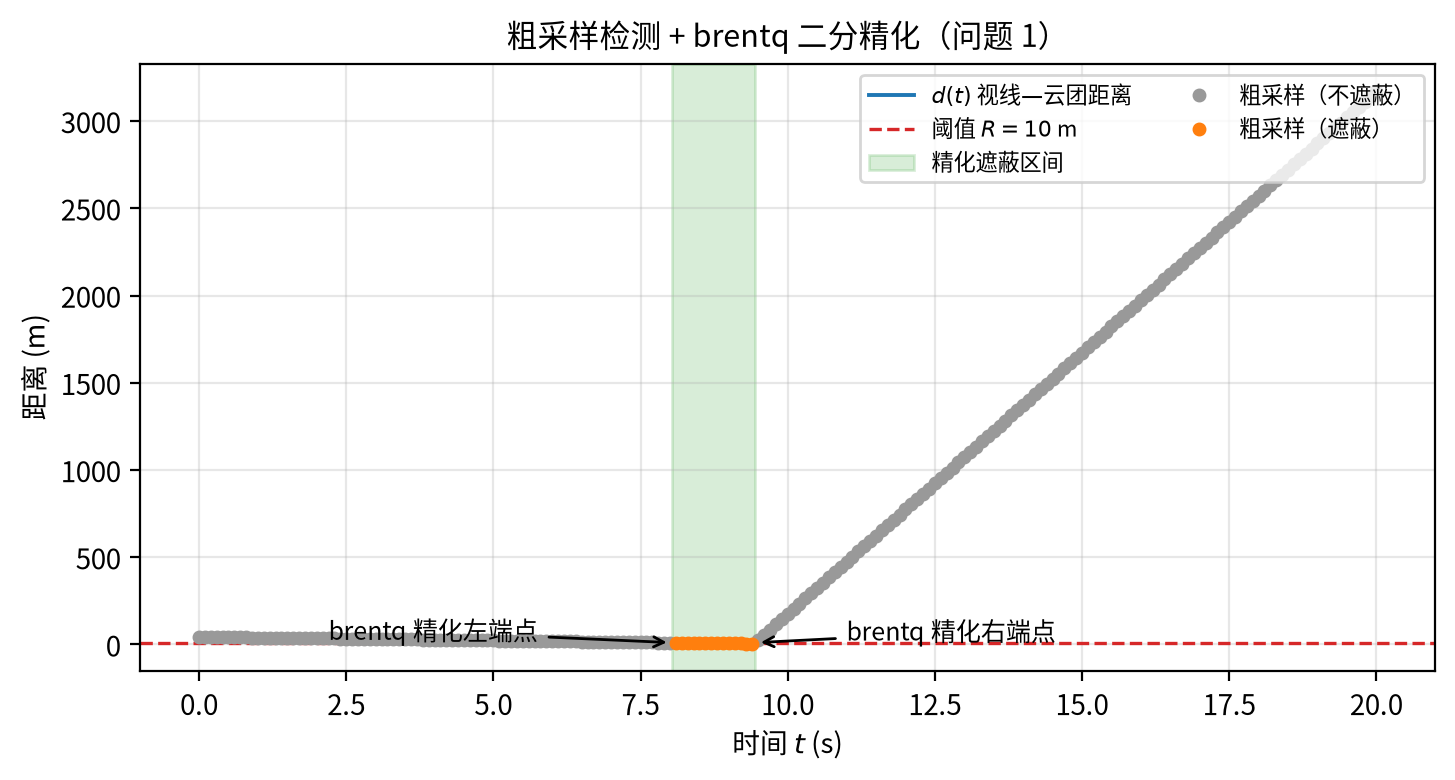
\includegraphics[width=0.78\textwidth]{fig5_interval_refine.png}
\caption{粗采样检测与 \texttt{brentq} 二分精化示意（问题 1：橙色圆点为粗采样遮蔽点，绿色区域为精化后的有效遮蔽区间）}
\label{fig:refine}
\end{figure}

\addtocontents{toc}{\protect\setcounter{tocdepth}{2}}
\subsection{结构化决策变量编码}
\addtocontents{toc}{\protect\setcounter{tocdepth}{1}}

模型四与模型六均涉及同机多弹投放间隔约束。设某无人机需投放 $n$ 枚弹，将原始变量 $u_1\le u_2\le\cdots\le u_n$ 排序后定义投放时刻
\begin{equation}
  t_{d1}=u_1,\qquad t_{d2}=u_2+1,\qquad \cdots,\qquad t_{dn}=u_n+(n-1),
  \label{eq:encoding}
\end{equation}
则任意两弹间隔自动满足
\begin{equation}
  t_{d(i+1)}-t_{di}=u_{i+1}-u_i+1\ge 1.
  \label{eq:gap}
\end{equation}
该编码的本质是把“时序约束”转化为“排序约束”：优化器只需在 $u$ 空间自由取值，而无需处理不可行投放时序。以问题 3 的最优解为例，排序变量与投放时刻的映射如表 \ref{tab:enc} 与图 \ref{fig:enc} 所示；引信延时 $\tau_j$ 按 $[0.5,\ \tau_{\max}(h_k)]$ 编码，天然保证式 \eqref{eq:height} 成立。各问题变量维度与含义见表 \ref{tab:dim}。

\begin{table}[H]
\centering
\caption{问题 3 的排序变量—投放时刻映射示例}
\label{tab:enc}
\small
\begin{tabular}{lccc}
\toprule
排序变量 $u_i$ & 0.0004 & 2.7189 & 3.5664 \\
投放时刻 $t_{di}=u_i+(i-1)$ & 0.0004 & 3.7189 & 5.5664 \\
与前弹间隔 (s) & --- & 3.7185 & 1.8475 \\
\bottomrule
\end{tabular}
\end{table}

\begin{figure}[H]
\centering
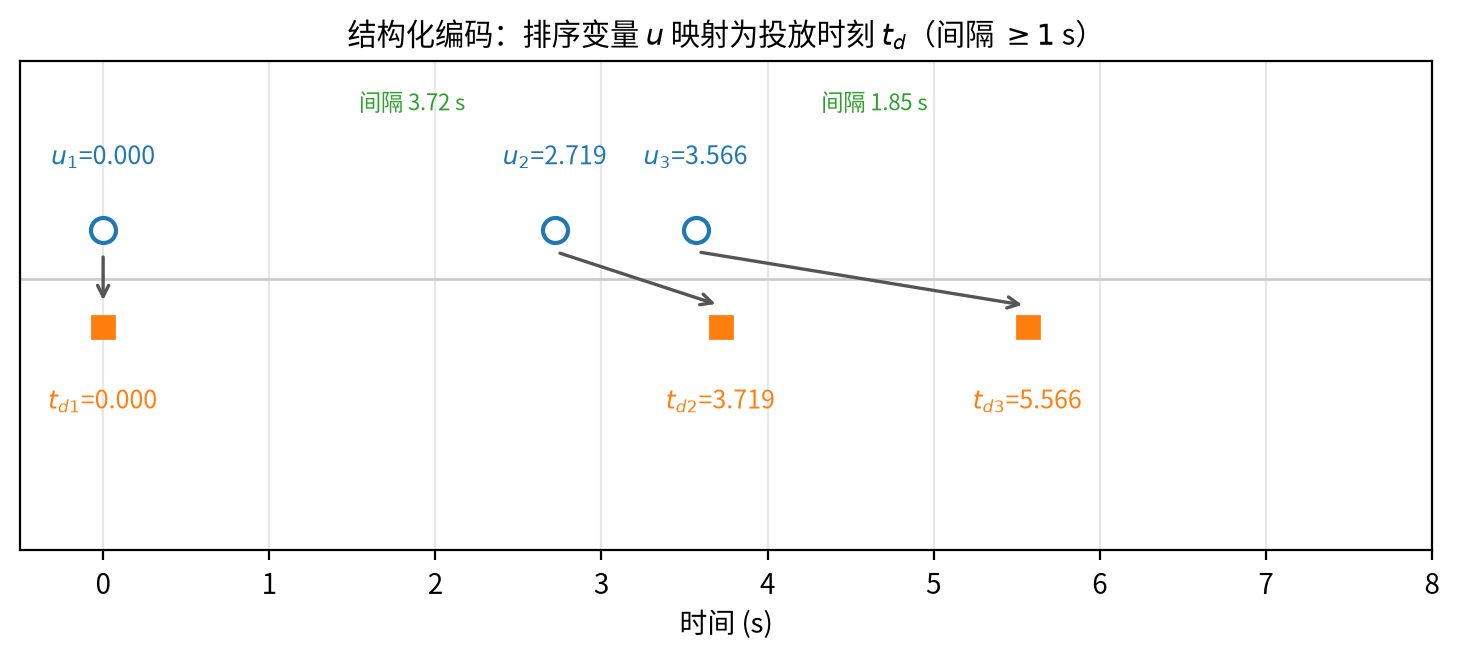
\includegraphics[width=0.72\textwidth]{fig5_encoding.png}
\caption{排序变量 $u$ 到投放时刻 $t_d$ 的结构化编码示意}
\label{fig:enc}
\end{figure}

\begin{table}[H]
\centering
\caption{各问题决策变量维度}
\label{tab:dim}
\begin{tabular}{lcl}
\toprule
问题 & 维度 & 变量说明 \\
\midrule
Q2 & 4 & FY1 的 $\theta,v,t_d,\tau$ \\
Q3 & 8 & FY1 的 $\theta,v$ + 3 弹的 $t_d,\tau$（排序编码） \\
Q4 & 12 & FY1--FY3 各 4 个独立变量 \\
Q5 & 40 & 5 机 $\times(\theta,v)$ + 15 弹 $\times(t_d,\tau)$（机内排序编码） \\
\bottomrule
\end{tabular}
\end{table}

\addtocontents{toc}{\protect\setcounter{tocdepth}{2}}
\subsection{几何启发式初始解构造}
\addtocontents{toc}{\protect\setcounter{tocdepth}{1}}

高维 DE 的收敛质量严重依赖初始种群。本文利用问题的几何结构构造可行种子：对任意“无人机 $k$—导弹 $m$”组合，给定目标起爆时刻 $t_b$ 与视线比例 $\lambda\in(0,1)$，取期望起爆点
\begin{equation}
  \bm{E}^{\mathrm{des}}=\bm{P}_m(t_b)+\lambda\left(\bm{T}-\bm{P}_m(t_b)\right),
  \label{eq:desired}
\end{equation}
即把云团放在“导弹—目标”视线上的指定位置。由式 \eqref{eq:height} 反推引信延时
\begin{equation}
  \tau=\sqrt{\frac{2\left(h_k-E^{\mathrm{des}}_z\right)}{g}},
  \label{eq:heur_tau}
\end{equation}
再令航向指向 $\bm{E}^{\mathrm{des}}$ 的水平投影方向，并在速度集 $\{70,90,110,130,140\}$ 中枚举，由水平距离反推投放时刻
\begin{equation}
  t_d=\frac{\left\|\bm{E}^{\mathrm{des}}_{xy}-\bm{U}_{k0,xy}\right\|}{v_k}-\tau.
  \label{eq:heur_td}
\end{equation}
只有当 $t_d\ge 0$、$\tau$ 在合法区间且起爆高度不小于 $60~\mathrm{m}$ 时才保留该种子。对 $t_b$ 取 $4\sim55~\mathrm{s}$ 的 18 个候选、$\lambda$ 取 6 个候选，可生成数百个可行解；再按目标值排序，取最优者作为 DE 初始种群的几何部分，其余位置由均匀随机样本填充。该方法同时用于问题 2--5，是保证 DE 从“可行且较优”区域起步的关键。

\begin{figure}[H]
\centering
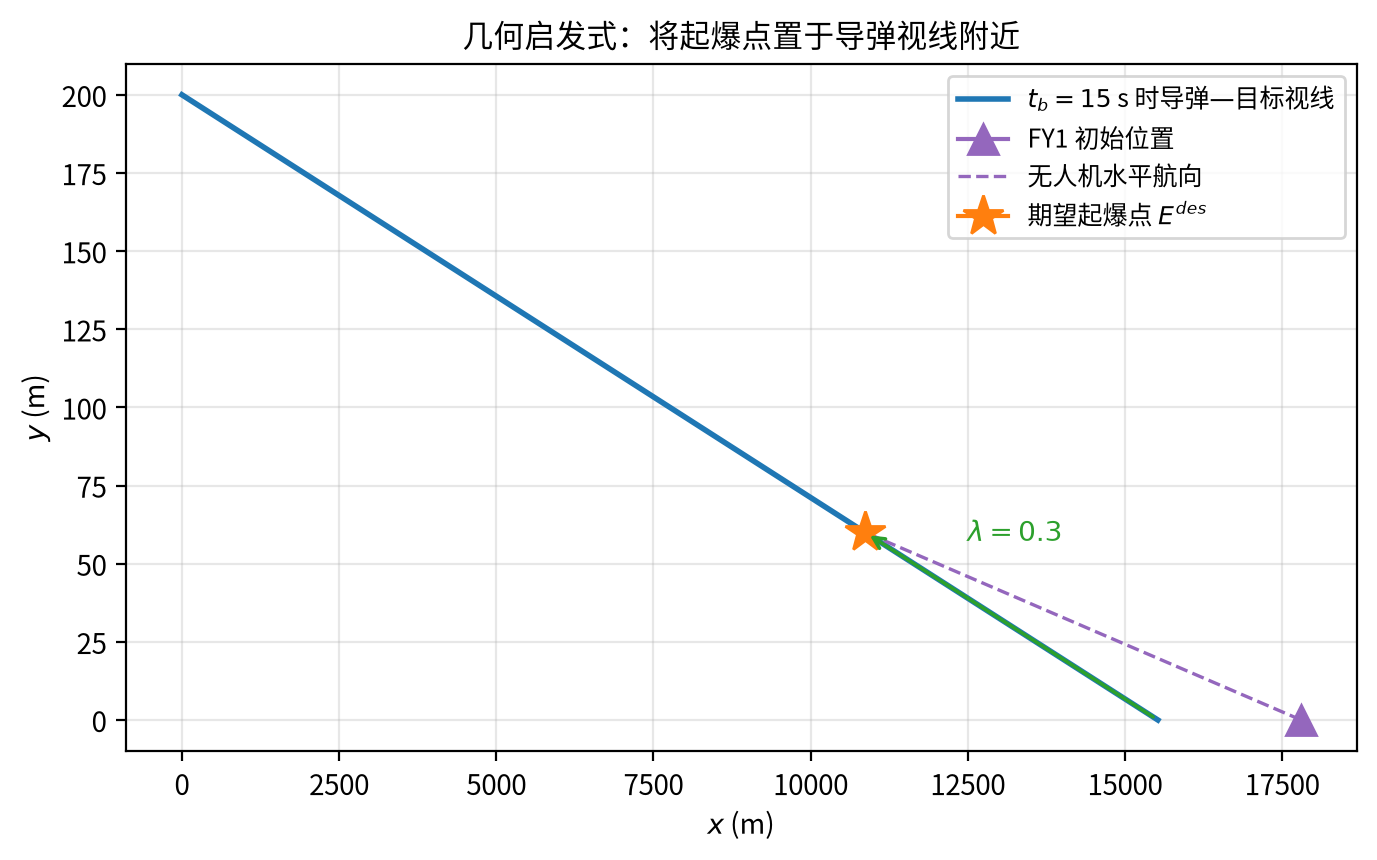
\includegraphics[width=0.66\textwidth]{fig5_heuristic.png}
\caption{几何启发式：将期望起爆点放在“导弹—目标”视线上，再反推无人机航向、速度与投放时刻}
\label{fig:heur}
\end{figure}

式 \eqref{eq:desired} 中 $\lambda$ 控制云团在视线上的前后位置，$t_b$ 控制遮蔽发生的时刻，二者共同决定云团的空间—时间坐标；式 \eqref{eq:heur_tau} 保证起爆高度合法，式 \eqref{eq:heur_td} 保证投放时刻非负。三个公式构成一个从“期望遮蔽时空点”到“投放参数”的闭合反演，能够以极小成本批量生成高质初始解。

\addtocontents{toc}{\protect\setcounter{tocdepth}{2}}
\subsection{CPU 差分进化与局部精修}
\addtocontents{toc}{\protect\setcounter{tocdepth}{1}}

问题 2--4 采用带启发式初始种群的差分进化（DE）求解。初始种群构造分三步：
\begin{enumerate}
  \item 几何启发种子：将起爆点置于“导弹—目标”视线附近的不同时刻，反推无人机航向、速度、投放时刻与引信延时，生成可行且较优的初始解；
  \item 随机样本：在变量边界内用拉丁超立方或均匀采样补充种群；
  \item 择优填充：对所有候选按目标值排序，取前 $P$ 个作为 DE 初始种群。
\end{enumerate}
DE 采用 rand/1/bin 变异策略与二项交叉。设第 $g$ 代种群为 $\{\bm{x}_i^{(g)}\}$，对每个个体随机选取三个互异基向量 $\bm{x}_a^{(g)},\bm{x}_b^{(g)},\bm{x}_c^{(g)}$，变异向量为
\begin{equation}
  \bm{v}_i^{(g+1)}=\bm{x}_a^{(g)}+F\left(\bm{x}_b^{(g)}-\bm{x}_c^{(g)}\right),
  \label{eq:mutation}
\end{equation}
其中 $F$ 为缩放因子。随后执行二项交叉生成试验向量：
\begin{equation}
  u_{i,j}^{(g+1)}=
  \begin{cases}
    v_{i,j}^{(g+1)}, & \mathrm{rand}_j\le C_r\ \text{或}\ j=j_{\mathrm{rand}},\\
    x_{i,j}^{(g)}, & \text{其他},
  \end{cases}
  \label{eq:crossover}
\end{equation}
其中 $C_r$ 为交叉率，$j_{\mathrm{rand}}$ 为随机选取的必交叉维度。选择算子按目标值择优：
\begin{equation}
  \bm{x}_i^{(g+1)}=
  \begin{cases}
    \bm{u}_i^{(g+1)}, & f\left(\bm{u}_i^{(g+1)}\right)\le f\left(\bm{x}_i^{(g)}\right),\\
    \bm{x}_i^{(g)}, & \text{其他}.
  \end{cases}
  \label{eq:selection}
\end{equation}
迭代结束后依次执行 L-BFGS-B 与带边界映射的 Nelder-Mead 局部精修。局部搜索的目标函数将越界变量映射回边界，避免优化器利用越界区域产生虚假最优。各问题的 DE 超参数如表 \ref{tab:de_params} 所示，随机种子统一取 2025。

\begin{table}[H]
\centering
\caption{各问题 DE 超参数}
\label{tab:de_params}
\small
\begin{tabular}{lcccccc}
\toprule
问题 & 算法 & 种群规模 & 迭代次数 & $F$ & $C_r$ & 种子 \\
\midrule
Q2 & SciPy DE & 20 & 800 & 0.5--1.0（抖动） & 0.7 & 2025 \\
Q3 & SciPy DE & 16 & 500 & 0.5--1.0（抖动） & 0.7 & 2025 \\
Q4 & SciPy DE & 14 & 500 & 0.5--1.0（抖动） & 0.7 & 2025 \\
Q5 & GPU 批量 DE & 16 & 600 & 0.75 & 0.9 & 2025 \\
\bottomrule
\end{tabular}
\end{table}

\addtocontents{toc}{\protect\setcounter{tocdepth}{2}}
\subsection{Triton 批量 GPU 差分进化}
\addtocontents{toc}{\protect\setcounter{tocdepth}{1}}

问题 5 的 40 维目标函数包含 $15$ 弹 $\times$ $3$ 导弹 $\times$ $700$ 个时间采样点的距离计算，单次 CPU 评估约 $1.4~\mathrm{ms}$，种群级评估成为主要瓶颈。为此，本文用 Triton 编写批量目标函数核函数：每个 CUDA 程序负责一个候选解与一枚导弹，将 $15$ 枚弹的云团参数解码后，在固定时间网格上向量化计算“点—线段距离”，并按导弹取并集，单次核函数调用即可评估整个 DE 种群。

记候选解 $b$ 的第 $j$ 枚弹对导弹 $m$ 在采样时刻 $t_k=k\Delta t$ 的遮蔽指示为
\begin{equation}
  I_{jm}^{(b)}(t_k)=\mathbf{1}\left\{d_{jm}^{(b)}(t_k)\le R,\ t_k\in W_{jm}^{(b)}\right\},
  \label{eq:indicator}
\end{equation}
其中 $W_{jm}^{(b)}$ 为云团有效期与导弹飞行窗口的交集。程序 $(b,m)$ 计算导弹 $m$ 的粗粒度遮蔽时长
\begin{equation}
  T_m^{(b)}=\Delta t\sum_{k=0}^{N-1}\left[\bigvee_{j=1}^{15} I_{jm}^{(b)}(t_k)\right],
  \label{eq:kernel}
\end{equation}
其中 $\bigvee$ 表示逻辑或，等价于按导弹对 15 枚弹取并集；主机端再对三枚导弹求和得到候选解的目标值 $E_b=-\sum_m T_m^{(b)}$。核函数网格与数据流如图 \ref{fig:kern} 所示，关键实现参数见表 \ref{tab:kern}。

\begin{figure}[H]
\centering
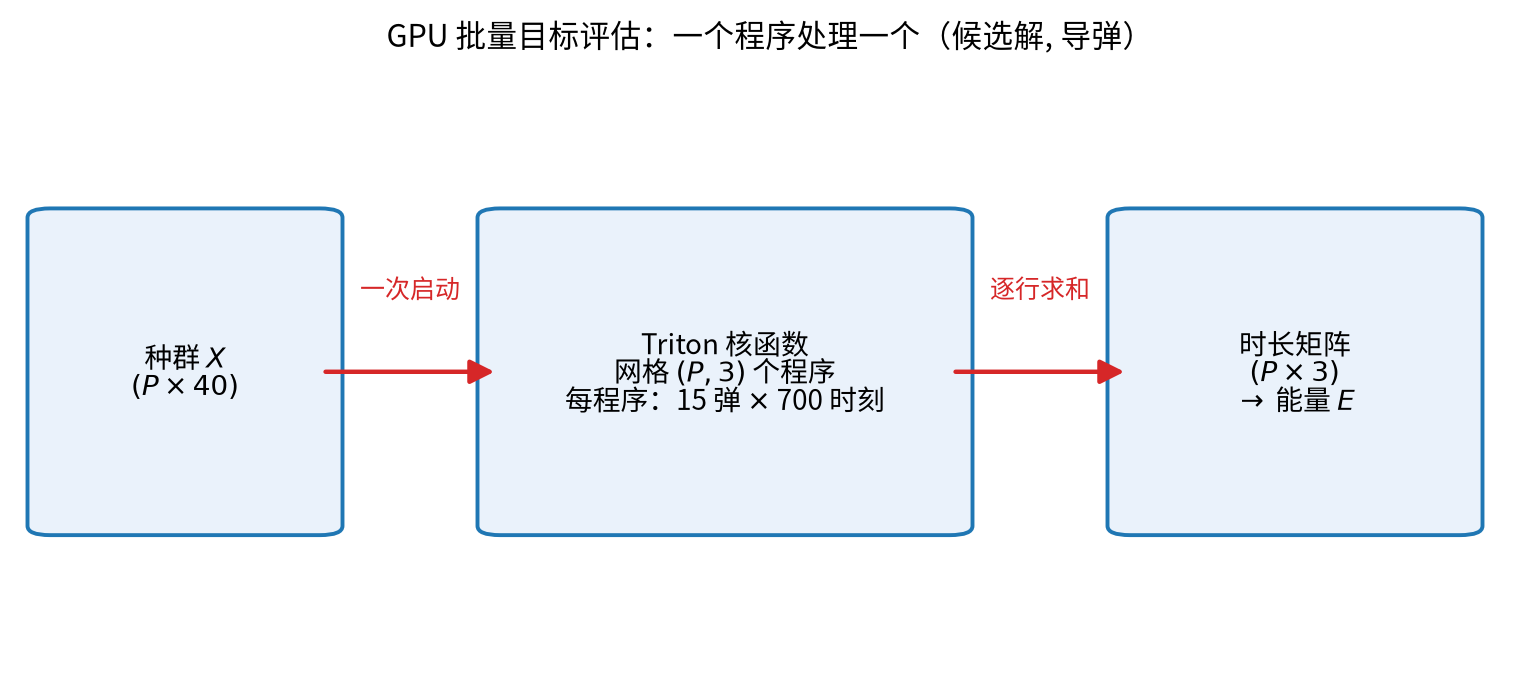
\includegraphics[width=0.86\textwidth]{fig5_gpu_kernel.png}
\caption{Triton 批量目标评估：网格 $(P,3)$ 中每个程序独立计算一个（候选解, 导弹）对的遮蔽时长}
\label{fig:kern}
\end{figure}

\begin{table}[H]
\centering
\caption{Triton 核函数关键参数}
\label{tab:kern}
\small
\begin{tabular}{lcl}
\toprule
参数 & 值 & 说明 \\
\midrule
$N$ & 700 & 固定时间网格 $0\sim70$ s，$\Delta t=0.1$ s \\
$\mathrm{BLOCK\_T}$ & 128 & 每个时间块并行处理的采样点数 \\
网格 & $(P,3)$ & $P$ 个候选解 $\times$ 3 枚导弹 \\
每程序负载 & $15\times700$ & 15 枚弹在 700 个时刻的点—线段距离 \\
单代距离计算量 & $\approx 19.7\times10^6$ & $P\times 3\times 15\times 700$（$P=624$） \\
\bottomrule
\end{tabular}
\end{table}

算法 2 给出 GPU 批量 DE 流程。

\begin{algorithm}[H]
\caption{GPU 批量差分进化（Q5）}
\label{alg:gpude}
\KwIn{变量边界；种群规模 $P$；迭代次数 $N_{\max}$；交叉率 $C_r$；缩放因子 $F$}
\KwOut{最优策略 $\bm{x}^*$ 与目标值}
\Begin{
  用几何启发种子与随机样本初始化种群 $\bm{X}$；
  \texttt{TritonKernel}$(\bm{X})$ 一次评估全部候选，得能量向量 $\bm{E}$；
  \For{$g=1,\dots,N_{\max}$}{
    对每个个体选择互异基向量 $\bm{x}_a,\bm{x}_b,\bm{x}_c$；
    $\bm{v}\leftarrow\bm{x}_a+F(\bm{x}_b-\bm{x}_c)$，并裁剪到边界；
    按 $C_r$ 与随机维度执行二项交叉，生成试验种群 $\bm{U}$；
    \texttt{TritonKernel}$(\bm{U})$ 评估试验能量 $\bm{E}_U$；
    选择：$\bm{E}_U<\bm{E}$ 时替换；
    精英保留最优个体并记录历史。
  }
  \Return 最优解 $\bm{x}^*$（再经 CPU 精化）
}
\end{algorithm}

实测 $624$ 个候选解的一代评估约 $0.5~\mathrm{ms}$，较 CPU 顺序评估加速约三个数量级。核函数实现中需特别注意时间索引的数据类型：将整数格点显式转换为浮点秒后再与云团寿命窗口比较，避免整数截断造成寿命误判。

为量化加速效果，表 \ref{tab:perf} 给出问题 5 优化过程中 CPU 与 GPU 的关键性能指标。可以看出，GPU 批量核函数把“每代种群评估”从亚秒级压缩到亚毫秒级，使得 40 维 DE 在可接受时间内完成 600 代迭代；总求解时间中主要开销已由目标评估转移至 DE 的变异、交叉与局部精修。

\begin{table}[H]
\centering
\caption{问题 5 CPU 与 GPU 求解性能对比}
\label{tab:perf}
\small
\begin{tabular}{lcc}
\toprule
指标 & CPU（NumPy 顺序） & GPU（Triton 批量） \\
\midrule
单次候选评估 & $\approx 1.4~\mathrm{ms}$ & --- \\
单代种群评估（624 候选） & $\approx 0.65~\mathrm{s}$ & $\approx 0.5~\mathrm{ms}$ \\
单代加速比 & --- & $\approx 1300\times$ \\
Q5 全流程墙钟时间 & 约 5 min & 约 2 min 17 s \\
\bottomrule
\end{tabular}
\end{table}

\addtocontents{toc}{\protect\setcounter{tocdepth}{2}}
\subsection{算法复杂度分析}
\addtocontents{toc}{\protect\setcounter{tocdepth}{1}}

设弹数为 $J$、导弹数为 $M$、时间采样点数为 $N$、DE 种群规模为 $B$、迭代次数为 $G$。各环节复杂度如表 \ref{tab:complexity} 所示。CPU 遮蔽区间算法的单次评估复杂度为 $O(JMN)$，其中距离计算与区间合并均向量化；DE 总评估次数为种群规模与迭代次数之积。GPU 批量版本将单次评估的 $O(JMN)$ 计算并行化到 $BM$ 个 CUDA 程序中，单代核函数启动开销约为 $0.5~\mathrm{ms}$，时间复杂度与种群规模近似解耦，适合高维问题的长时间迭代。

\begin{table}[H]
\centering
\caption{算法复杂度汇总}
\label{tab:complexity}
\small
\begin{tabular}{ll}
\toprule
环节 & 复杂度 \\
\midrule
CPU 单次目标评估 & $O(JMN)$ \\
多弹区间合并 & $O(K\log K)$，$K$ 为区间总数 \\
CPU DE 总评估 & $O(GBJMN)$ \\
GPU 单代评估 & $O(JMN)$ 并行于 $BM$ 个程序 \\
GPU 核函数显存 & $O(B\times 40 + B\times 3)$，距离矩阵不落地 \\
\bottomrule
\end{tabular}
\end{table}

\section{模型检验与灵敏度分析}

\addtocontents{toc}{\protect\setcounter{tocdepth}{2}}
\subsection{正确性验证}
\addtocontents{toc}{\protect\setcounter{tocdepth}{1}}

代码包含 13 项单元测试，覆盖点—线段距离三种几何情形、自由落体运动学、必遮蔽/必不遮蔽/半遮蔽场景、投放间隔编码与 xlsx 导出读回，全部通过。问题 1 的遮蔽区间由粗采样 + \texttt{brentq} 与 $0.005~\mathrm{s}$ 稠密采样交叉验证，端点误差小于 $0.01~\mathrm{s}$；所得区间 $[8.038,\ 9.448]~\mathrm{s}$ 与提示词参考值一致，验证了模型的物理实现。此外，GPU 粗粒度目标函数与 CPU 目标函数在 64 个随机策略上的最大总时长偏差为 $0.203~\mathrm{s}$，属于采样端点舍入差异，不影响优化方向。

对问题 5 最终策略，GPU 粗网格、CPU 粗网格与 CPU 精化三套评估的逐导弹时长分别为 M1：$12.1/11.8/12.145~\mathrm{s}$，M2：$4.8/4.7/4.855~\mathrm{s}$，M3：$3.9/3.9/3.947~\mathrm{s}$。GPU 与 CPU 粗网格偏差不超过 $0.3~\mathrm{s}$，粗网格与精化结果偏差不超过 $0.2~\mathrm{s}$，验证了“GPU 引导搜索、CPU 精化定值”两阶段流程的一致性。

\addtocontents{toc}{\protect\setcounter{tocdepth}{2}}
\subsection{参数扰动分析}
\addtocontents{toc}{\protect\setcounter{tocdepth}{1}}

对重力加速度 $g$（$9.8\to10$）、云团半径 $R$（$9/10/11~\mathrm{m}$）、最低起爆高度（$60\to30~\mathrm{m}$）及遮蔽判据（点目标 $\to$ 圆柱目标）进行扰动，各问题遮蔽时长变化如表 \ref{tab:sens} 所示。

\begin{table}[H]
\centering
\caption{关键参数扰动下的遮蔽时长（s）}
\label{tab:sens}
\small
\resizebox{\textwidth}{!}{%
\begin{tabular}{lcccccc}
\toprule
 & 基准 & $g=10.0$ & $R=9.0$ & $R=11.0$ & 最低起爆高 30 m & 圆柱判据 \\
\midrule
Q1 & 1.410 & 1.673 & 1.166 & 1.652 & 1.410 & 1.392 \\
Q2 & 4.667 & 4.564 & 4.200 & 4.891 & 4.667 & 4.537 \\
Q3 & 7.740 & 7.310 & 6.766 & 8.029 & 7.740 & 7.614 \\
Q4 & 14.335 & 13.453 & 12.903 & 14.815 & 14.335 & 11.343 \\
Q5 & 20.947 & 10.673 & 18.794 & 21.914 & 20.947 & 16.021 \\
\bottomrule
\end{tabular}}
\end{table}

可以看出：云团半径增大 $1~\mathrm{m}$ 时各问题遮蔽时长约增加 $0.1\sim1.0~\mathrm{s}$，呈单调正相关；圆柱判据使 Q4、Q5 分别下降约 $3.0~\mathrm{s}$、$4.9~\mathrm{s}$，说明目标几何细节对多弹协同结果影响较大；$g$ 的扰动对 Q5 影响最明显，这是因为起爆点随弹道整体偏移。总体而言，模型对半径与重力的响应方向符合物理直觉，结论稳健。图 \ref{fig:sens3d} 给出 Q2 与 Q5 最优策略在 $(g,R)$ 双参数扰动下的三维响应曲面。

从相对变化率看，$R=9.0$ 时各问题下降约 $7\%\sim10\%$，$R=11.0$ 时上升约 $5\%\sim17\%$，变化幅度与云团半径近似线性；圆柱判据对 Q4、Q5 的影响（约 $-21\%$、$-24\%$）显著大于单机模型，说明当云团需要同时遮挡圆柱表面多个视线方向时，多弹布设的空间覆盖要求更高。

\begin{figure}[H]
\centering
\begin{subfigure}[b]{0.48\textwidth}
  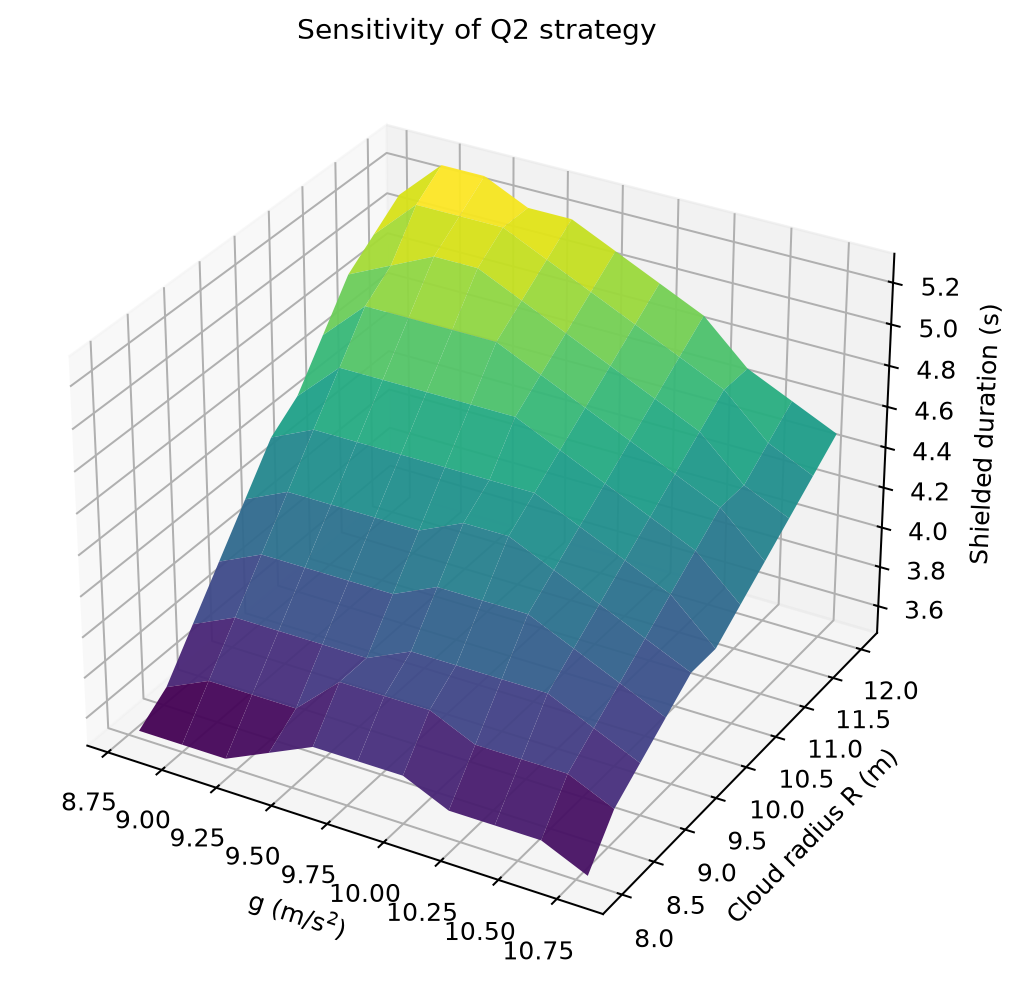
\includegraphics[width=\textwidth]{fig_sens3d_q2.png}
  \caption{Q2 响应曲面}
\end{subfigure}
\hfill
\begin{subfigure}[b]{0.48\textwidth}
  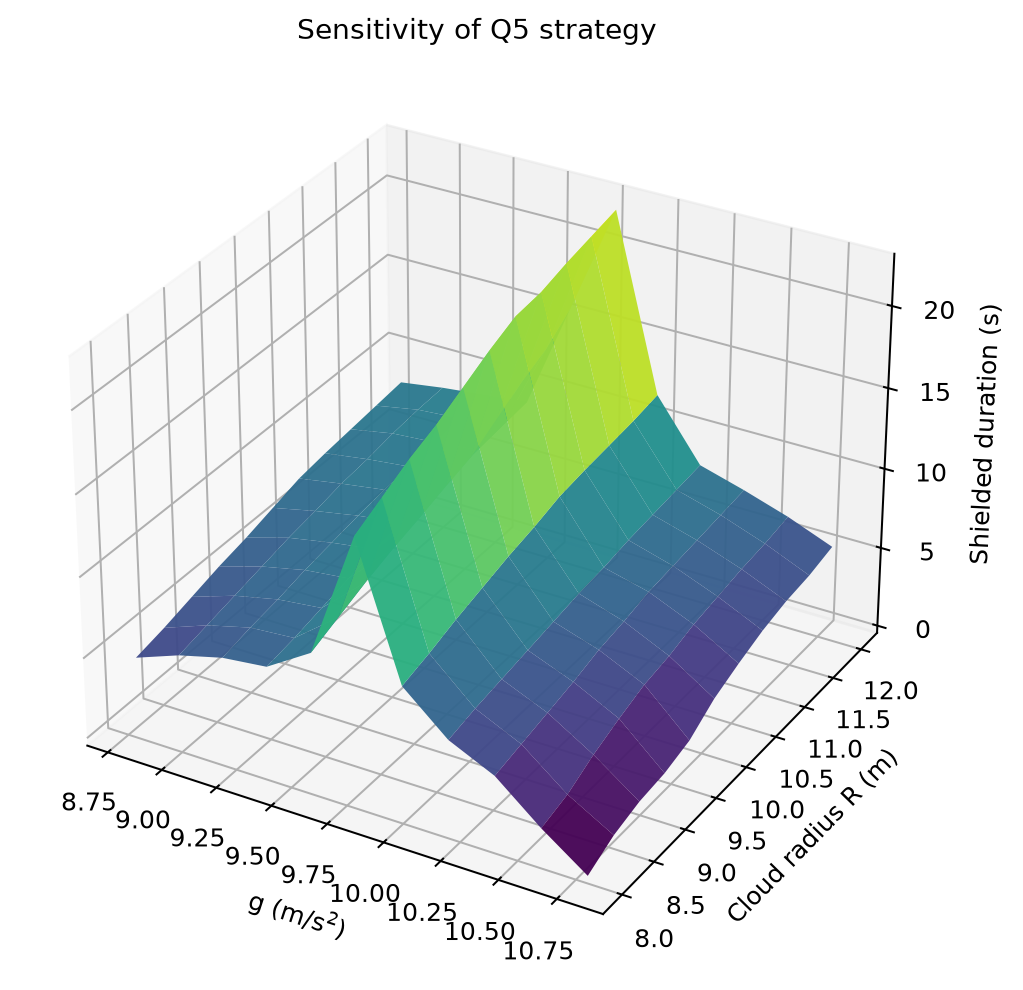
\includegraphics[width=\textwidth]{fig_sens3d_q5.png}
  \caption{Q5 响应曲面}
\end{subfigure}
\caption{遮蔽时长对重力加速度 $g$ 与云团半径 $R$ 的耦合灵敏度}
\label{fig:sens3d}
\end{figure}

\addtocontents{toc}{\protect\setcounter{tocdepth}{2}}
\subsection{收敛性与稳健性}
\addtocontents{toc}{\protect\setcounter{tocdepth}{1}}

所有优化均固定随机种子 2025，两次运行结果完全一致。问题 2--4 的 DE 收敛曲线在迭代后期进入平台，表明种群已收敛；问题 5 采用 GPU 批量 DE 迭代 600 代，目标值从初始可行解持续提升并最终稳定在 $20.9~\mathrm{s}$ 附近。局部精修阶段将粗网格解切换为 \texttt{brentq} 精化目标后，各问题遮蔽时长仅发生 $10^{-2}\sim10^{-1}~\mathrm{s}$ 量级变化，说明优化结果对网格精度不敏感。

为验证区间算法的数值稳定性，将粗网格 + \texttt{brentq} 与 $0.005~\mathrm{s}$ 稠密采样对比：问题 1 区间分别为 $[8.0379,9.4481]~\mathrm{s}$ 与 $[8.0400,9.4450]~\mathrm{s}$，问题 2 区间分别为 $[2.7094,7.3763]~\mathrm{s}$ 与 $[2.7144,7.3744]~\mathrm{s}$。两种方法端点误差均小于 $0.01~\mathrm{s}$，遮蔽时长差异小于 $0.01~\mathrm{s}$，表明主算法在保证计算效率的同时具有足够精度。

\section{结果分析与讨论}

\addtocontents{toc}{\protect\setcounter{tocdepth}{2}}
\subsection{问题 1：固定策略直接计算}
\addtocontents{toc}{\protect\setcounter{tocdepth}{1}}

\textbf{问题分析：}FY1 的航向、速度、投放时刻与引信延时全部给定，属于模型一与模型二的直接应用，无需优化。

\textbf{求解与验证：}FY1 以 $120~\mathrm{m/s}$ 朝向假目标飞行，$t=1.5~\mathrm{s}$ 投放、$3.6~\mathrm{s}$ 后起爆。计算得投放点 $(17620.00,\allowbreak 0.00,\allowbreak 1800.00)$，起爆点 $(17188.00,\allowbreak 0.00,\allowbreak 1736.50)$，M1 的有效遮蔽区间为 $[8.038,\allowbreak 9.448]~\mathrm{s}$，遮蔽时长 $T_1=1.410~\mathrm{s}$。图 \ref{fig:q1} 给出遮蔽区间与三维轨迹。

\begin{figure}[H]
\centering
\begin{subfigure}[b]{0.46\textwidth}
  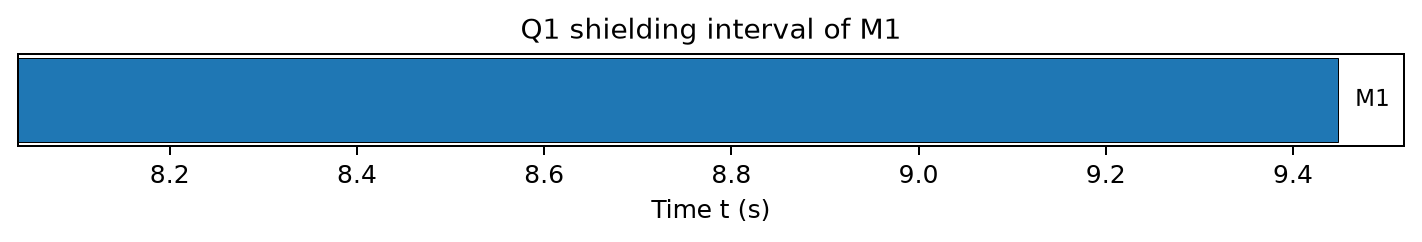
\includegraphics[width=\textwidth]{q1_gantt.png}
  \caption{遮蔽区间}
\end{subfigure}
\hfill
\begin{subfigure}[b]{0.5\textwidth}
  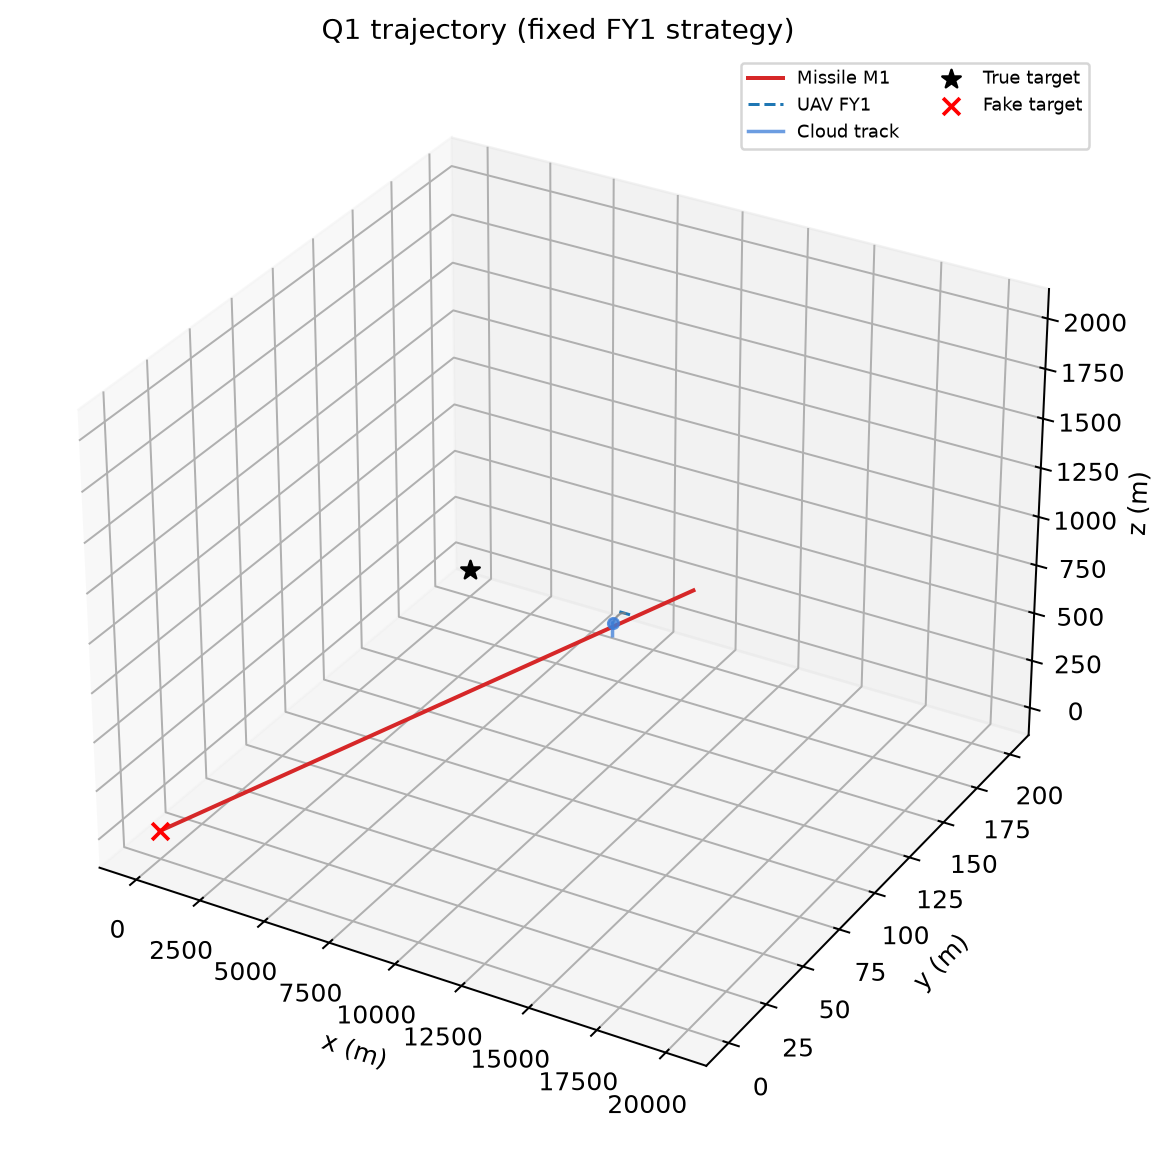
\includegraphics[width=\textwidth]{q1_traj3d.png}
  \caption{三维轨迹}
\end{subfigure}
\caption{问题 1 计算结果}
\label{fig:q1}
\end{figure}

\addtocontents{toc}{\protect\setcounter{tocdepth}{2}}
\subsection{问题 2：FY1 单弹优化}
\addtocontents{toc}{\protect\setcounter{tocdepth}{1}}

\textbf{问题分析：}问题 2 为模型三的 4 维连续优化，目标函数无解析梯度，采用 DE 全局搜索 + 多起点局部精修。

\textbf{求解与验证：}最优策略及遮蔽结果已按提交格式列于表 \ref{tab:q2}（第 4 节），遮蔽时长达 $T_1=4.667~\mathrm{s}$，为问题 1 的 $3.31$ 倍。遮蔽区间为 $[2.709,\allowbreak 7.376]~\mathrm{s}$。图 \ref{fig:q2} 给出区间、轨迹与收敛曲线。

\begin{figure}[H]
\centering
\begin{subfigure}[b]{0.30\textwidth}
  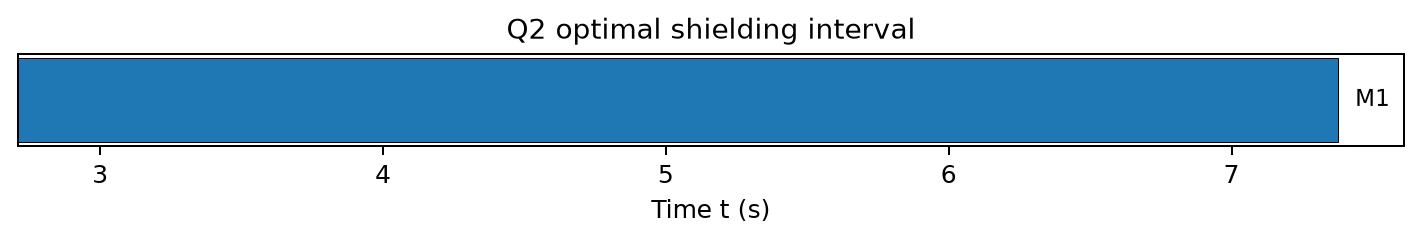
\includegraphics[width=\textwidth]{q2_gantt.png}
  \caption{遮蔽区间}
\end{subfigure}
\hfill
\begin{subfigure}[b]{0.34\textwidth}
  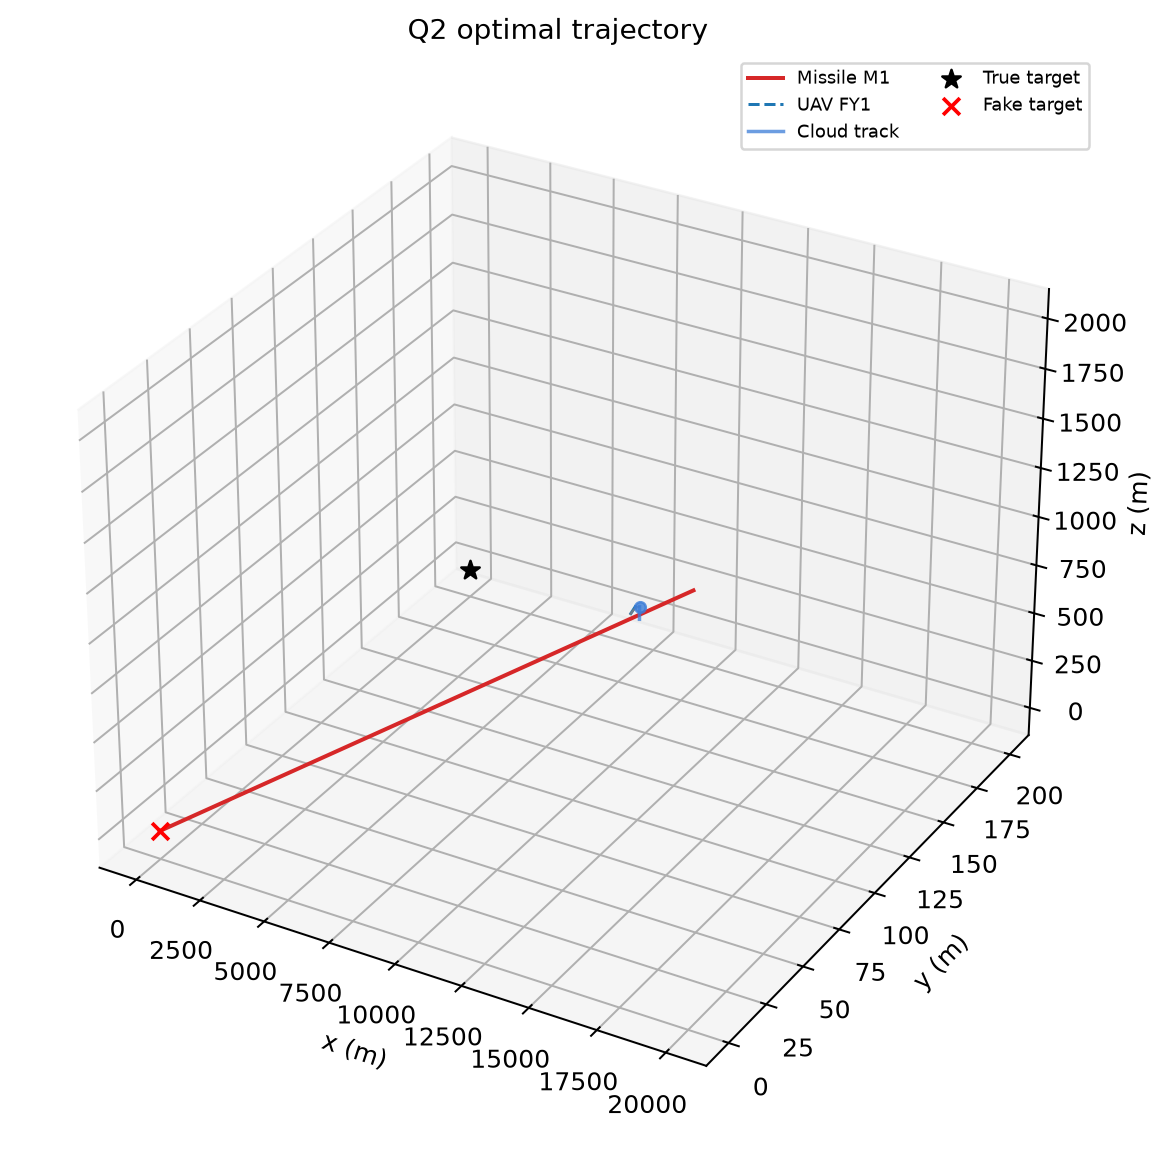
\includegraphics[width=\textwidth]{q2_traj3d.png}
  \caption{三维轨迹}
\end{subfigure}
\hfill
\begin{subfigure}[b]{0.26\textwidth}
  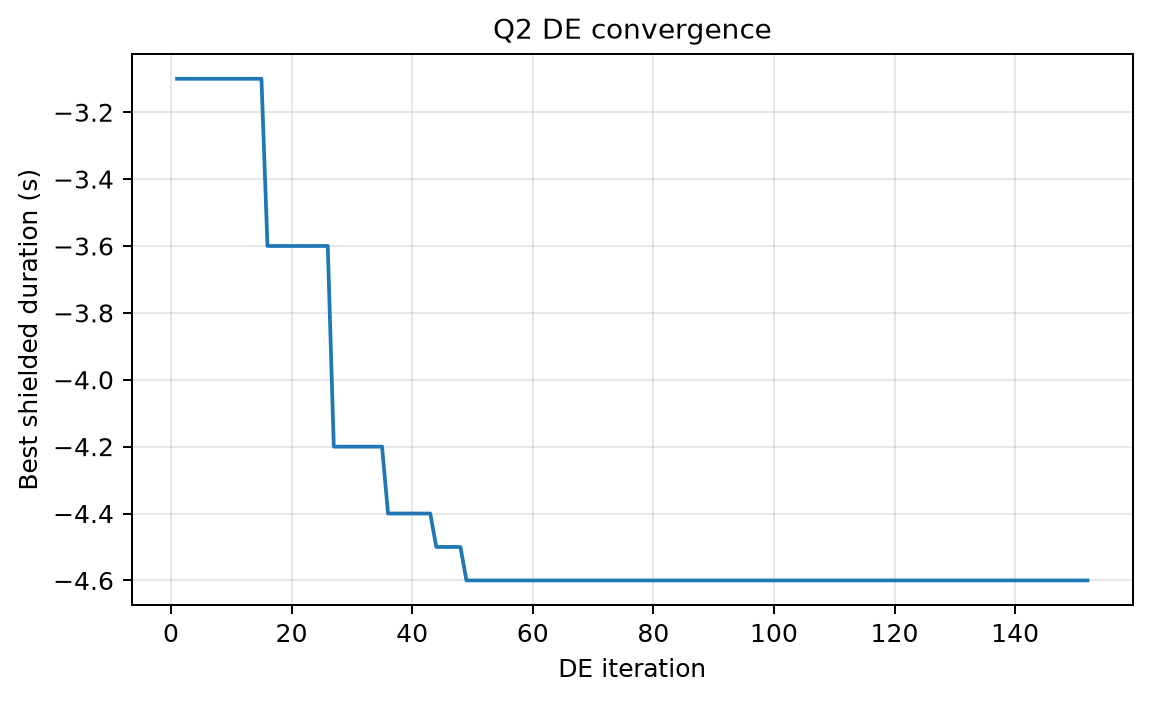
\includegraphics[width=\textwidth]{q2_convergence.png}
  \caption{收敛曲线}
\end{subfigure}
\caption{问题 2 优化结果}
\label{fig:q2}
\end{figure}

\addtocontents{toc}{\protect\setcounter{tocdepth}{2}}
\subsection{问题 3：FY1 三弹优化}
\addtocontents{toc}{\protect\setcounter{tocdepth}{1}}

\textbf{问题分析：}问题 3 为模型四的 8 维联合优化，三弹共享航向与速度，机内投放时序由式 \eqref{eq:spacing} 编码，天然满足间隔约束。

\textbf{求解与验证：}FY1 以 $\theta_1=3.135~\mathrm{rad}$、$v_1=140~\mathrm{m/s}$ 飞行，三弹投放时刻分别为 $0.000,\allowbreak 3.719,\allowbreak 5.566~\mathrm{s}$。三弹遮蔽区间依次衔接，并集时长达 $T_1=7.740~\mathrm{s}$（区间 $[5.077,\allowbreak 12.816]~\mathrm{s}$），单弹贡献分别为 $3.921,\allowbreak 2.612,\allowbreak 1.206~\mathrm{s}$。详细策略已按 \texttt{result1.xlsx} 格式列于表 \ref{tab:q3}（第 4 节），图 \ref{fig:q3} 给出三维轨迹。

\begin{figure}[H]
\centering
\begin{subfigure}[b]{0.42\textwidth}
  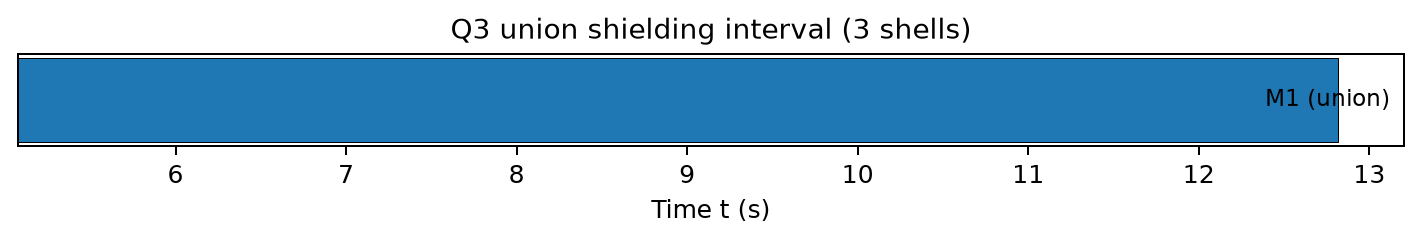
\includegraphics[width=\textwidth]{q3_gantt.png}
  \caption{并集遮蔽区间}
\end{subfigure}
\hfill
\begin{subfigure}[b]{0.46\textwidth}
  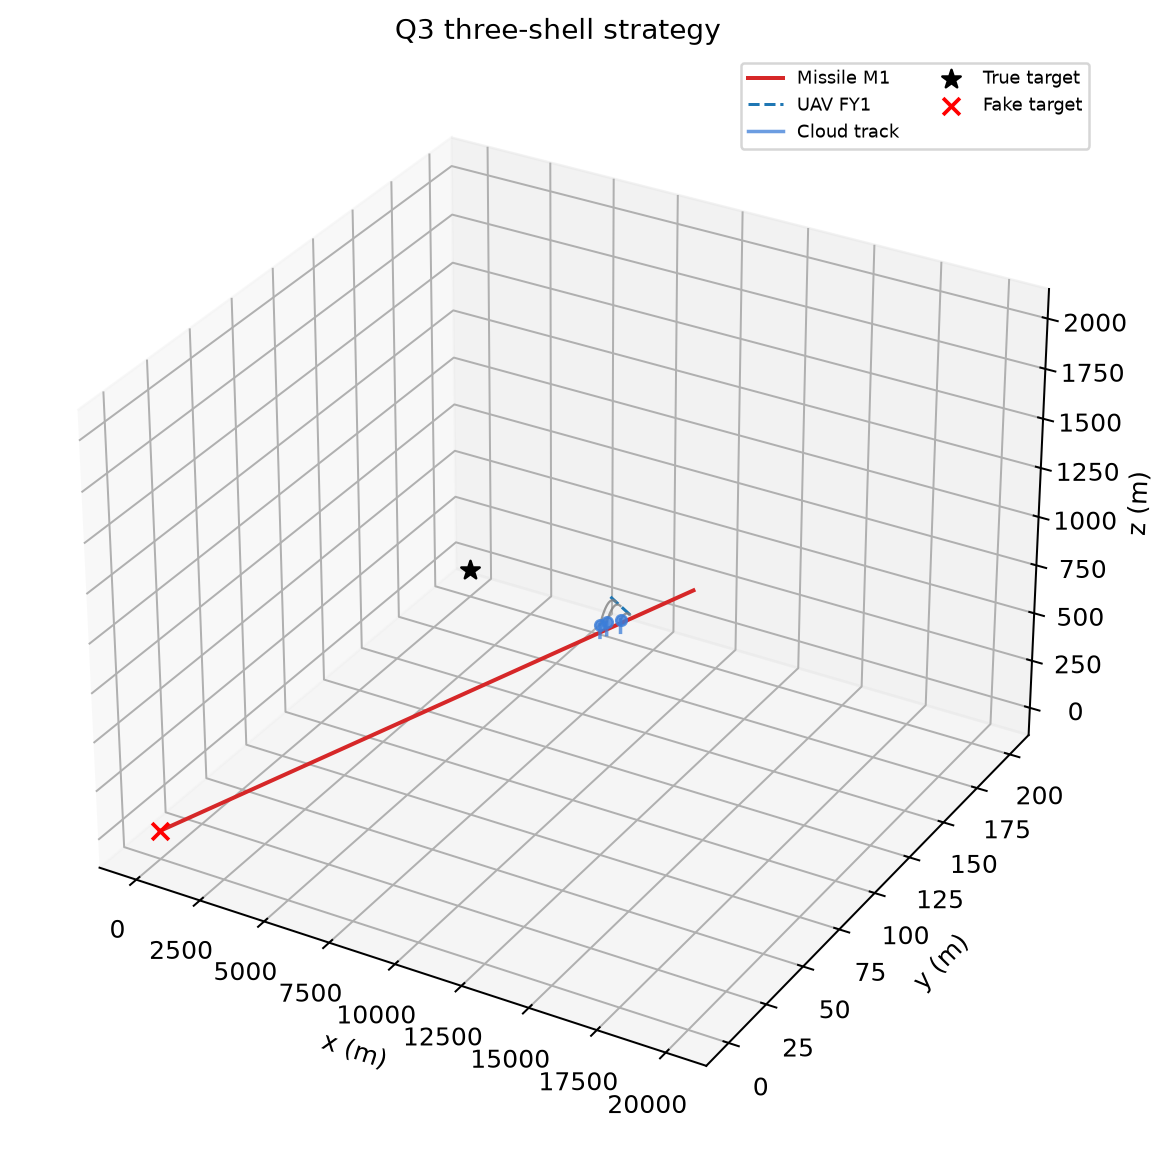
\includegraphics[width=\textwidth]{q3_traj3d.png}
  \caption{三弹三维轨迹}
\end{subfigure}
\caption{问题 3 优化结果}
\label{fig:q3}
\end{figure}

\addtocontents{toc}{\protect\setcounter{tocdepth}{2}}
\subsection{问题 4：三机各一弹优化}
\addtocontents{toc}{\protect\setcounter{tocdepth}{1}}

\textbf{问题分析：}问题 4 为模型五的 12 维联合优化，三架无人机变量完全独立，不存在机间时序耦合。

\textbf{求解与验证：}最优策略已按 \texttt{result2.xlsx} 格式列于表 \ref{tab:q4}（第 4 节）。三弹遮蔽区间分别为 $[5.458,\allowbreak 9.935]$、$[12.609,\allowbreak 17.192]$、$[22.194,\allowbreak 27.469]~\mathrm{s}$，相互衔接，并集时长达 $T_1=14.335~\mathrm{s}$。

\begin{figure}[H]
\centering
\begin{subfigure}[b]{0.42\textwidth}
  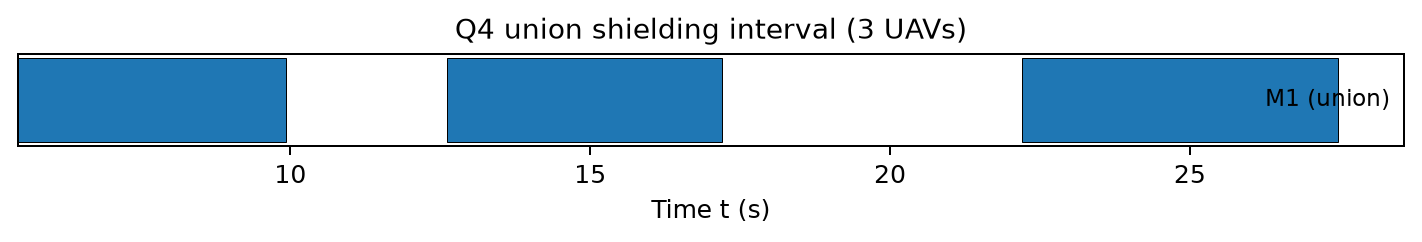
\includegraphics[width=\textwidth]{q4_gantt.png}
  \caption{并集遮蔽区间}
\end{subfigure}
\hfill
\begin{subfigure}[b]{0.46\textwidth}
  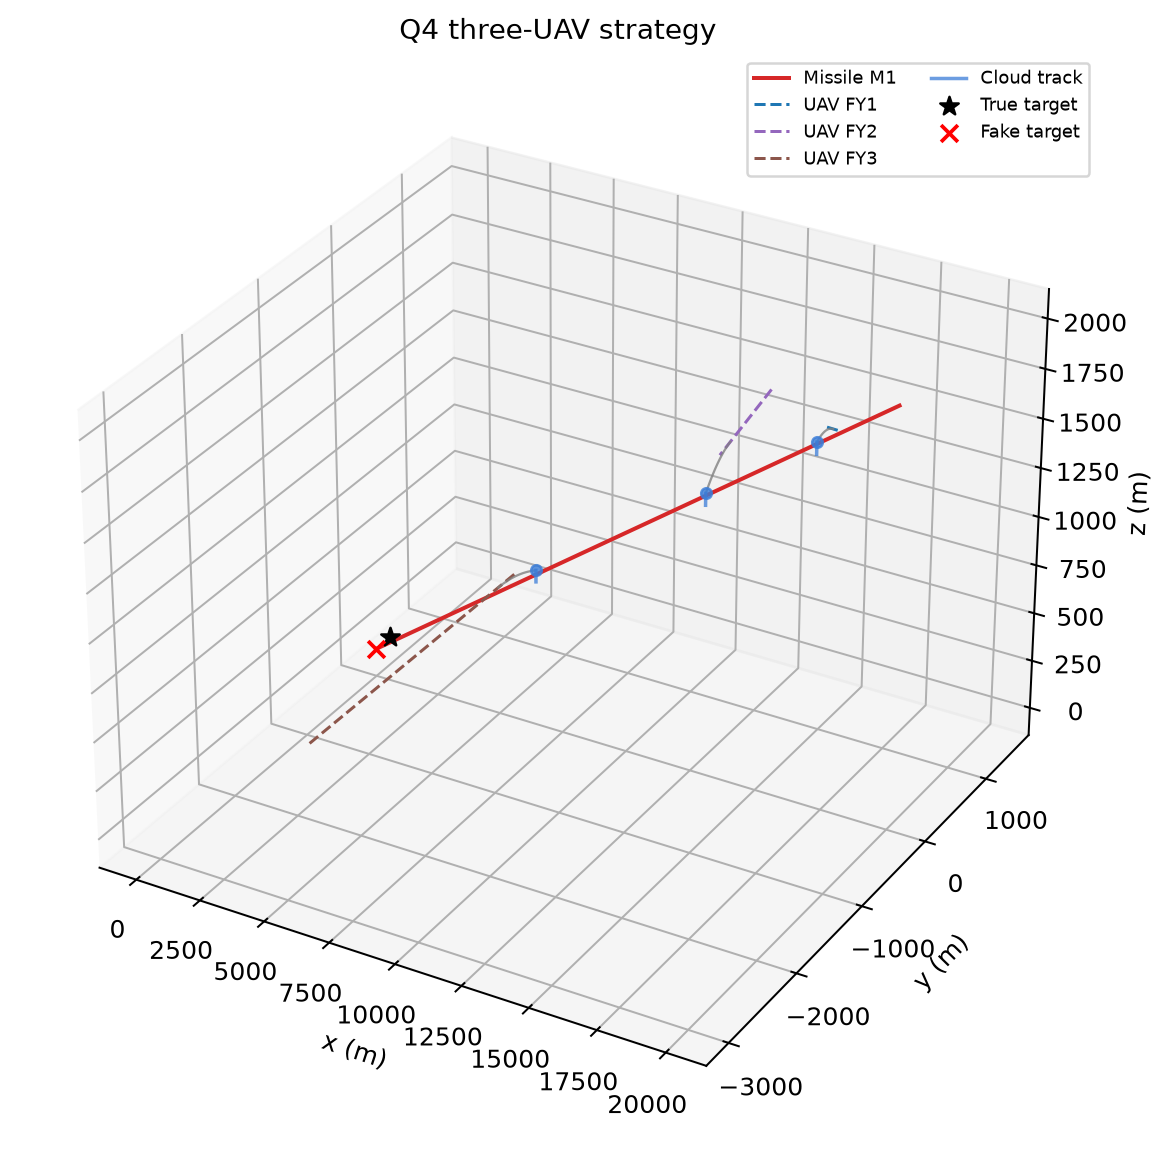
\includegraphics[width=\textwidth]{q4_traj3d.png}
  \caption{三机三维轨迹}
\end{subfigure}
\caption{问题 4 优化结果}
\label{fig:q4}
\end{figure}

\addtocontents{toc}{\protect\setcounter{tocdepth}{2}}
\subsection{问题 5：五机十五弹全局优化}
\addtocontents{toc}{\protect\setcounter{tocdepth}{1}}

\textbf{问题分析：}问题 5 为模型六的 40 维全局优化，同时存在弹—导弹分配、机内投放时序与跨导弹资源竞争三类耦合，是本文计算量最大的模型。

\textbf{求解与验证：}采用每架无人机 3 弹、分别对应 M1--M3 的满配方案，以 GPU 批量 DE 迭代 600 代并经 CPU 精化。最终总遮蔽时长 $T_{\mathrm{sum}}=20.947~\mathrm{s}$，其中 M1、M2、M3 分别为 $12.145~\mathrm{s}$、$4.855~\mathrm{s}$、$3.947~\mathrm{s}$，最差导弹遮蔽时长为 $3.947~\mathrm{s}$；三枚导弹同时被遮蔽的时长为 $0~\mathrm{s}$，说明烟幕资源在时间上呈错峰布置。导弹级结果已按 \texttt{result3.xlsx} 格式列于表 \ref{tab:q5}（第 4 节），完整 15 弹投放参数见附录表 \ref{tab:q5full} 与 \texttt{result3.xlsx}。

\begin{figure}[H]
\centering
\begin{subfigure}[b]{0.42\textwidth}
  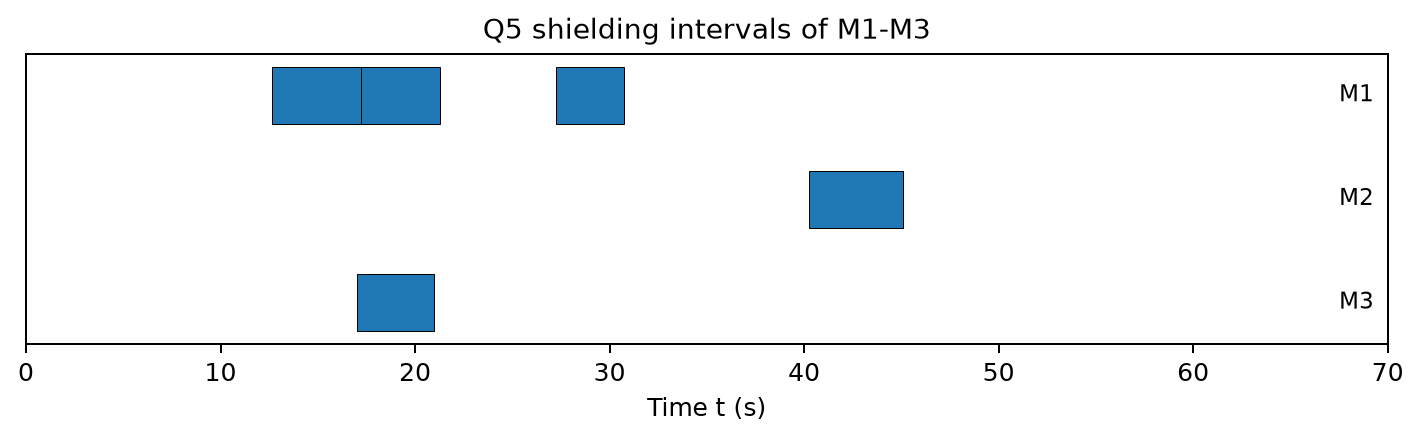
\includegraphics[width=\textwidth]{q5_gantt.png}
  \caption{三导弹遮蔽区间}
\end{subfigure}
\hfill
\begin{subfigure}[b]{0.46\textwidth}
  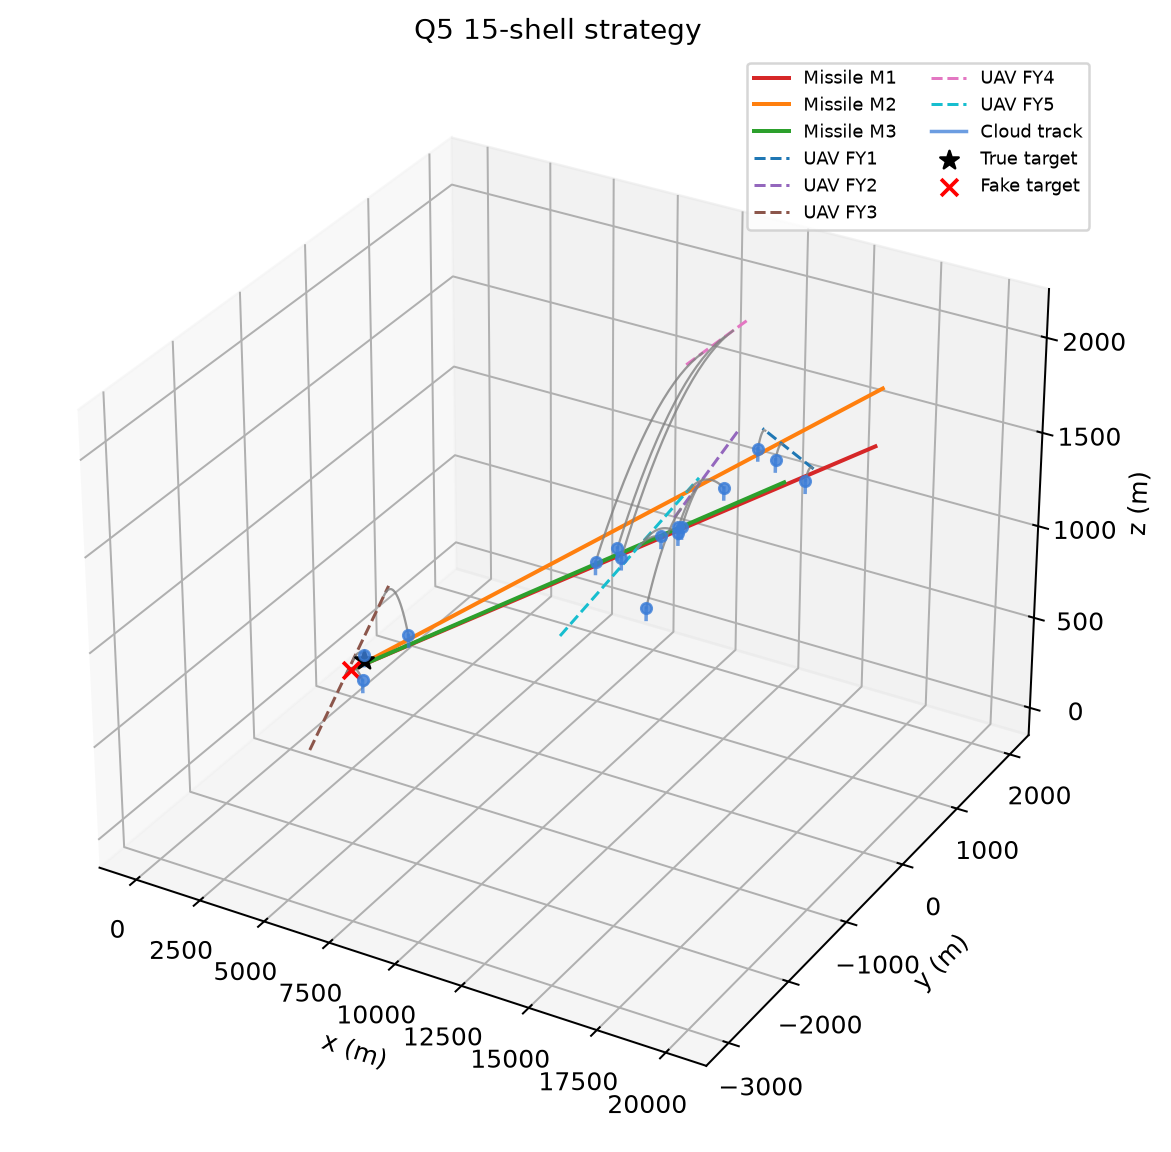
\includegraphics[width=\textwidth]{q5_traj3d.png}
  \caption{15 弹三维轨迹}
\end{subfigure}
\caption{问题 5 优化结果}
\label{fig:q5}
\end{figure}

\begin{figure}[H]
\centering
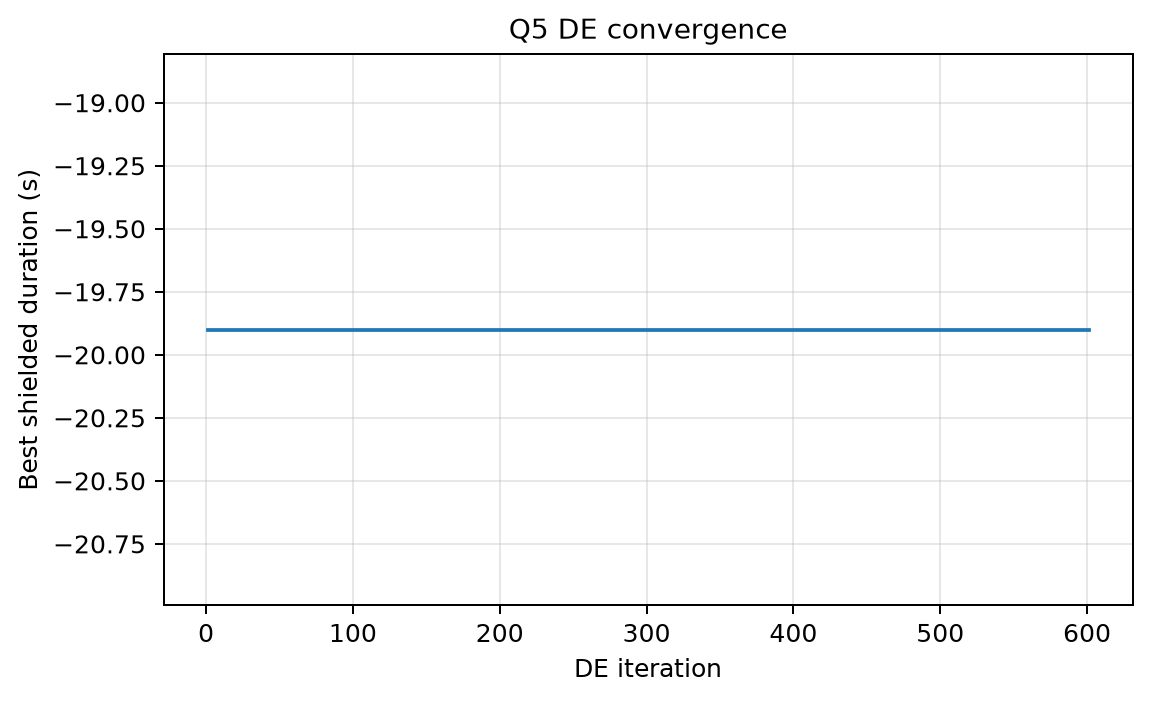
\includegraphics[width=0.55\textwidth]{q5_convergence.png}
\caption{问题 5 GPU 批量 DE 收敛曲线}
\label{fig:q5conv}
\end{figure}

\subsection{结果综合讨论}

从问题 1 到问题 4，单目标遮蔽时长由 $1.410~\mathrm{s}$ 增至 $14.335~\mathrm{s}$，说明弹数与投放时机协同能够有效拼接遮蔽区间。问题 5 中 M1 获得 3 个遮蔽区间、M2 与 M3 各 1 个，总时长达 $20.947~\mathrm{s}$；最差导弹仍有约 $3.9~\mathrm{s}$ 的连续遮蔽窗口，可在实战中为告警与机动争取时间。

进一步分析资源分配结构可以发现：三枚导弹到达假目标的时刻依次为 $67.0~\mathrm{s}$（M1）、$63.8~\mathrm{s}$（M2）、$60.4~\mathrm{s}$（M3），M1 的可用遮蔽窗口最长，因此优化器将更多弹分配给 M1；M2 与 M3 各获得一个连续窗口。该结果与“最大化总遮蔽时长”的目标函数一致。若实际任务要求三弹同时致盲，可将式 \eqref{eq:metrics} 中的 $T_{\mathrm{sim}}$ 或 $T_{\mathrm{worst}}$ 作为目标函数的加权项，此时资源分配将向均衡方向移动，但总遮蔽时长会有所下降。

\subsection{问题间对比与边际收益}

为量化各问题规模扩张带来的收益，表 \ref{tab:compare} 汇总五个问题的资源规模、遮蔽时长与相对问题 1 的倍数。

\begin{table}[H]
\centering
\caption{各问题结果汇总与相对增益}
\label{tab:compare}
\small
\begin{tabular}{lcccccc}
\toprule
问题 & 无人机数 & 弹数 & 目标导弹数 & 遮蔽时长 (s) & 相对问题 1 倍数 \\
\midrule
Q1 & 1 & 1 & 1 & 1.410 & 1.00 \\
Q2 & 1 & 1 & 1 & 4.667 & 3.31 \\
Q3 & 1 & 3 & 1 & 7.740 & 5.49 \\
Q4 & 3 & 3 & 1 & 14.335 & 10.17 \\
Q5 & 5 & 15 & 3 & 20.947 & 14.85 \\
\bottomrule
\end{tabular}
\end{table}

从边际收益看：Q2 相对 Q1 的增益为 $+3.257~\mathrm{s}$；Q3 增加 2 弹后进一步增加 $3.073~\mathrm{s}$；Q4 通过三机异构布局实现 $6.595~\mathrm{s}$ 的最大单步增幅；Q5 虽将弹数扩至 15 枚，但需同时服务 3 枚导弹，总时长仅再增加 $6.612~\mathrm{s}$，平均每弹贡献约 $1.40~\mathrm{s}$，低于 Q3 的每弹 $2.58~\mathrm{s}$。这说明目标从“单目标连续遮蔽”转向“多目标错峰覆盖”后边际收益递减，符合预期；若按每枚导弹平均遮蔽时长衡量，Q5 为 $6.98~\mathrm{s}$，仍显著高于单目标方案，体现了多机协同的总体优势。

\section{结论}

本文针对烟幕干扰弹投放策略问题，建立了从运动学方程到几何遮蔽判定的完整数学模型，并按问题复杂度分别建立了单弹优化模型、同机多弹协同模型、多机协同模型与多机多弹多导弹全局优化模型，设计了粗采样 + 二分精化算法与结构化变量编码，并针对问题 5 的 40 维优化实现 Triton 批量 GPU 差分进化。

五个问题的有效遮蔽时长依次为 $1.410~\mathrm{s}$、$4.667~\mathrm{s}$、$7.740~\mathrm{s}$、$14.335~\mathrm{s}$ 与 $20.947~\mathrm{s}$，结果经单元测试、稠密采样交叉验证与参数扰动分析检验。未来可在以下方向扩展：考虑导弹末端机动与风场扰动下的鲁棒策略；引入多目标优化同时最大化总遮蔽时长与最差导弹遮蔽时长；将烟幕浓度扩散模型纳入遮蔽判定；以及将投放策略推广到更多无人机与动态目标场景。

从工程实施角度，本文给出三点建议：第一，问题 5 的最优策略中多数弹的实际贡献为 0，实际部署时可先按贡献遮蔽区间筛选“有效弹”，将冗余弹留作备份或在后续时刻补投，以提高弹药利用率；第二，三枚导弹同时遮蔽时长为 0，若防御方需要在某一关键时刻同时致盲三枚导弹，应把 $T_{\mathrm{sim}}$ 作为目标函数的一项并以加权方式权衡总时长；第三，模型对重力加速度和云团半径较敏感，实战中应结合当日气象与弹种实测数据对 $g$、$R$ 进行在线标定，再按本文框架重算投放策略，以保证决策的实时有效性。

\section{模型评价}

\subsection{优点}
\begin{itemize}
  \item 模型严格建立在题目给定的确定性运动学上，不引入额外假设，物理含义清晰、可解释性强；
  \item 按问题逐级建立独立模型，决策变量、目标与约束边界清楚，便于逐题验证与扩展；
  \item 遮蔽区间采用“粗采样 + \texttt{brentq}”算法，优化阶段计算高效、最终结果精度高；
  \item 结构化编码把同机投放间隔硬约束融入变量空间，避免罚函数调参；
  \item Triton GPU 批量评估使 40 维问题的大规模差分进化成为可能，代码可复现、可扩展；
  \item 通过单元测试、稠密采样交叉验证与敏感性分析形成了完整验证链。
\end{itemize}

\subsection{不足}
\begin{itemize}
  \item 云团被简化为几何球体，未考虑烟幕浓度随时间的扩散与衰减；
  \item 导弹、无人机均为理想匀速直线运动，未考虑机动、风场与定位误差；
  \item 问题 5 的 40 维优化依赖启发式初始化与全局 DE，理论上仍不能保证全局最优；
  \item 三弹同时遮蔽时长为 0，若实际任务要求“同时致盲”，需将最差导弹遮蔽或同时遮蔽时长纳入目标函数。
\end{itemize}

\begin{thebibliography}{99}
\bibitem{cumcm2025} 全国大学生数学建模竞赛组委会. 2025 年高教社杯全国大学生数学建模竞赛 A 题：烟幕干扰弹的投放策略[EB/OL]. (2025).
\bibitem{smoke} 姚禄玖, 高钧麟, 李澄俊, 等. 烟幕理论与应用技术[M]. 北京: 国防工业出版社, 2004.
\bibitem{storn1997} Storn R, Price K. Differential evolution—a simple and efficient heuristic for global optimization over continuous spaces[J]. Journal of Global Optimization, 1997, 11(4): 341-359.
\bibitem{virtanen2020} Virtanen P, Gommers R, Oliphant T E, et al. SciPy 1.0: fundamental algorithms for scientific computing in Python[J]. Nature Methods, 2020, 17(3): 261-272.
\bibitem{triton2019} Tillet P, Kung H T, Cox D. Triton: an intermediate language and compiler for tiled neural network computations[C]//Proceedings of the 3rd ACM SIGPLAN International Workshop on Machine Learning and Programming Languages. 2019: 10-19.
\bibitem{mathmodel} 司守奎, 孙玺菁. 数学建模算法与应用[M]. 北京: 国防工业出版社, 2015.
\end{thebibliography}

\appendix
\section{附录：实现与数据说明}

\subsection{代码结构}

求解代码位于竞赛工作目录 \texttt{2025\_cumcm\_A} 下，模块职责单一：\texttt{geometry.py} 实现点—线段距离与区间代数；\texttt{kinematics.py} 实现式 (1)--(5) 的运动学；\texttt{shielding.py} 实现遮蔽区间主算法；\texttt{objective.py} 实现变量编解码与目标函数；\texttt{triton\_objective.py} 实现 GPU 批量目标核函数；\texttt{optimize\_gpu.py} 实现 GPU 批量 DE；\texttt{problems.py} 为 Q1--Q5 求解入口；\texttt{export.py} 导出三个 xlsx。运行 \texttt{scripts/run\_all.py} 可一键复现全部结果。

\subsection{结果文件与列字段说明}

按题干要求，问题 3、4、5 的结果分别写入 \texttt{result1.xlsx}、\texttt{result2.xlsx}、\texttt{result3.xlsx}。\texttt{result1.xlsx} 与 \texttt{result2.xlsx} 各 3 行，字段为弹编号、无人机、速度、航向角、投放时刻、起爆时刻、投放点 $x/y/z$、起爆点 $x/y/z$、单弹遮蔽时长；\texttt{result3.xlsx} 共 15 行，在前者基础上增加目标导弹、贡献遮蔽区间两列。由于当前工作目录未提供官方模板，三个文件按提示词第 9.2 节的默认列规范生成；若后续获得官方模板，可修改 \texttt{export.py} 中的列映射后重新导出。所有 xlsx 文件均通过 \texttt{pandas.read\_excel} 读回校验，行数与列名与 \texttt{results/q3\_best.json}、\texttt{q4\_best.json}、\texttt{q5\_best.json} 完全一致，数值保留 2--3 位小数。

\subsection{问题 5 完整投放策略}

问题 5 的 15 枚弹完整参数已写入 \texttt{result3.xlsx}，包括每弹对应的无人机、目标导弹、速度、航向角、投放/起爆时刻、投放/起爆点、贡献遮蔽区间与单弹遮蔽时长。表 \ref{tab:q5full} 给出全部参数，所有坐标单位均为米，时间单位为秒；数值与 \texttt{results/q5\_best.json} 逐位一致。

\begin{table}[H]
\centering
\caption{问题 5 完整投放策略（result3.xlsx）}
\label{tab:q5full}
\scriptsize
\resizebox{\textwidth}{!}{%
\begin{tabular}{ccccccccccccccc}
\toprule
弹编号 & 无人机 & 目标导弹 & 速度 $v~\mathrm{(m/s)}$ & 航向角 $\theta~\mathrm{(rad)}$ & 投放时刻 $t_d~\mathrm{(s)}$ & 起爆时刻 $t_e~\mathrm{(s)}$ & 投放点 $x$ & 投放点 $y$ & 投放点 $z$ & 起爆点 $x$ & 起爆点 $y$ & 起爆点 $z$ & 贡献遮蔽区间 (s) & 遮蔽时长 (s) \\
\midrule
1 & FY1 & M1 & 75.674 & 2.997 & 1.096 & 5.444 & 17717.93 & 11.93 & 1800.00 & 17392.32 & 59.25 & 1707.36 & --- & 0.000 \\
2 & FY1 & M2 & 75.674 & 2.997 & 22.039 & 26.701 & 16149.54 & 239.87 & 1800.00 & 15800.45 & 290.60 & 1693.52 & --- & 0.000 \\
3 & FY1 & M3 & 75.674 & 2.997 & 34.345 & 39.333 & 15228.03 & 373.80 & 1800.00 & 14854.46 & 428.09 & 1678.07 & --- & 0.000 \\
4 & FY2 & M1 & 129.981 & 5.299 & 8.053 & 12.628 & 12579.66 & 528.48 & 1400.00 & 12908.99 & 33.33 & 1297.44 & $[12.628,17.201]$ & 4.573 \\
5 & FY2 & M2 & 129.981 & 5.299 & 9.350 & 13.383 & 12673.04 & 388.09 & 1400.00 & 12963.39 & $-48.46$ & 1320.28 & --- & 0.000 \\
6 & FY2 & M3 & 129.981 & 5.299 & 12.891 & 20.383 & 12927.91 & 4.88 & 1400.00 & 13467.22 & $-805.96$ & 1124.96 & --- & 0.000 \\
7 & FY3 & M1 & 130.146 & 2.485 & 14.389 & 20.934 & 4517.26 & $-1856.12$ & 700.00 & 3842.85 & $-1335.84$ & 490.12 & --- & 0.000 \\
8 & FY3 & M2 & 130.146 & 2.485 & 17.401 & 21.699 & 4206.87 & $-1616.67$ & 700.00 & 3764.01 & $-1275.02$ & 609.49 & --- & 0.000 \\
9 & FY3 & M3 & 130.146 & 2.485 & 30.267 & 40.242 & 2881.11 & $-593.89$ & 700.00 & 1853.22 & 199.08 & 212.44 & --- & 0.000 \\
10 & FY4 & M1 & 140.000 & 4.480 & 1.591 & 14.141 & 10948.76 & 1783.27 & 1800.00 & 10544.48 & 73.33 & 1028.16 & --- & 0.000 \\
11 & FY4 & M2 & 140.000 & 4.480 & 2.591 & 14.578 & 10916.55 & 1647.03 & 1800.00 & 10530.42 & 13.85 & 1095.90 & --- & 0.000 \\
12 & FY4 & M3 & 140.000 & 4.480 & 5.140 & 17.018 & 10834.44 & 1299.73 & 1800.00 & 10451.83 & $-318.57$ & 1108.68 & $[17.018,20.965]$ & 3.947 \\
13 & FY5 & M1 & 130.241 & 1.969 & 12.830 & 16.886 & 12352.18 & $-459.67$ & 1300.00 & 12147.39 & 27.27 & 1219.39 & $[17.201,21.282]$ & 4.081 \\
14 & FY5 & M2 & 130.241 & 1.969 & 14.014 & 19.878 & 12292.39 & $-317.49$ & 1300.00 & 11996.31 & 386.49 & 1131.52 & --- & 0.000 \\
15 & FY5 & M3 & 130.241 & 1.969 & 21.522 & 28.073 & 11913.32 & 583.83 & 1300.00 & 11582.54 & 1370.33 & 1089.70 & --- & 0.000 \\
\bottomrule
\end{tabular}}
\end{table}

\subsection{复现命令}

\begin{verbatim}
python -m pytest tests -q
python scripts/run_q1.py
python scripts/run_q2.py
python scripts/run_q3.py
python scripts/run_q4.py
python scripts/run_q5.py
python scripts/run_sensitivity.py
python scripts/run_all.py
\end{verbatim}

依赖：Python 3.10+、NumPy、SciPy、Pandas、OpenPyXL、Matplotlib、PyTorch、Triton。随机种子固定为 2025。

\end{document}
